\documentclass[11pt,a4paper]{article}
\usepackage[margin=2.2cm]{geometry}
\usepackage{mathptmx}
\usepackage[expansion=false]{microtype}
\usepackage{amsmath}
\usepackage{amssymb}
\usepackage{graphicx}
\usepackage{booktabs}
\usepackage{array}
\usepackage[labelsep=period,font=small]{caption}
\usepackage[numbers,sort&compress]{natbib}
\usepackage{algorithm}
\usepackage{algpseudocode}
\usepackage{setspace}
\usepackage{xcolor}
\usepackage[hidelinks]{hyperref}
\setlength{\parskip}{0.35em}
% allow floats to be placed alongside the text instead of being deferred
\renewcommand{\topfraction}{0.92}
\renewcommand{\bottomfraction}{0.75}
\renewcommand{\textfraction}{0.06}
\renewcommand{\floatpagefraction}{0.72}
\setcounter{topnumber}{3}
\setcounter{bottomnumber}{2}
\setcounter{totalnumber}{4}
\newcommand{\method}{VAST-GWO}
\newcommand{\arc}{\mathcal{A}}
\newcommand{\sS}{\mathcal{S}}
\title{\bfseries \method{}: a verified archive-guided sparse-evaluation grey wolf
optimizer for global optimization and 3D UAV delivery path planning}
\author{}
\date{}

\begin{document}
\maketitle
\vspace{-1.6cm}

\begin{abstract}
\noindent
In black-box optimization the resource that decides solution quality is the
number of real objective evaluations, not the number of arithmetic operations.
The grey wolf optimizer (GWO) spends this resource uniformly over the whole
pack and derives all movement from three leaders, which invites premature
convergence and makes each evaluation less informative than it could be. This
paper proposes \method{}, a verified archive-guided sparse-evaluation GWO. In
every generation, 100 cheap candidates are generated from three complementary
routes: standard GWO leader moves (50), success-scale shells around the current
alpha wolf (12), and multi-region shells and two-centre segments produced from
a verified elite archive (38). Only $K=10$ uniformly sampled candidates receive
a real evaluation, and no unevaluated candidate ever influences leaders,
archives or rankings---a verified-state discipline that keeps every piece of
search memory backed by a billed evaluation. On CEC2017 at $D=50$ with
100{,}000 true evaluations and 30 independent runs, \method{} ranks first among
seven methods (mean rank 2.24), significantly outperforming the 2026
hierarchical HAGWO, PSO, CLPSO, the 2026 adaptive oppositional AOGWO and
standard GWO, and reaching statistical parity with the strong improved GWO
while leading it on mean rank. A controlled equal-slot ablation shows that the
verified archive carries the improvement: a GWO-only candidate pool loses 27
of the 29 functions to the full method, replacing the archive with a
single alpha-centred sampler with identical slots, scale and acceptance rule
collapses the method to 2 wins, and the alpha-shell route is optional once the
archive is present. Directed screening, fixed quotas and three Q-learning
schedulers were all rejected against matched controls, indicating that the
candidate-source structure, not the evaluation scheduler, is the decisive
design variable. In a 209-dimensional, DEM-based 3D UAV delivery application
with hard time windows, \method{} is the only method that finds feasible routes
in all 150 runs, attains the smallest censored mean time to feasibility, and
produces the best paired final route quality against every baseline after Holm
correction.
\end{abstract}

\vspace{0.2cm}
\noindent\textbf{Keywords:} grey wolf optimizer; sparse evaluation; verified
elite archive; multi-region search; limited evaluation budget; UAV path
planning; CEC2017.

\section{Introduction}
\label{sec:intro}
Nature-inspired optimizers are routinely used for engineering design,
scheduling and path planning because they assume little about the objective
and scale to black-box simulators. Their practical cost, however, is dominated
by the objective function itself. In finite-element calibration,
computational-fluid design or UAV mission planning a single evaluation may
take seconds to hours, so the total number of \emph{real} evaluations is the
binding constraint rather than the number of arithmetic operations
\citep{yu2021multimodel,liu2024survey,zhao2025surrogate}. Under such budgets an
optimizer has to answer one question well: \emph{where should the next real
evaluation be spent?}

The grey wolf optimizer (GWO) \citep{mirjalili2014gwo} is an attractive
starting point. It is parameter-light, easy to implement and has been applied
across the Internet of Things, feature selection, agriculture and UAV planning
\citep{nadimishahraki2024iot,makhadmeh2023review}. Its classic form, however,
evaluates the entire pack every generation and derives all movement from the
three leaders $\alpha$, $\beta$ and $\delta$. When evaluations are scarce this
design has two structural consequences. First, the search state is thin: apart
from the three leaders, the pack retains no memory of the regions it has
visited, so a region that produced a verified improvement but no current
leader is forgotten immediately. Second, the movement distribution contracts
around the same three attractors, which is the classical route to premature
convergence and stagnation on multimodal landscapes. Both effects are visible
in the behaviour of standard GWO on the CEC2017 suite and are documented across
the GWO literature \citep{makhadmeh2023review,nadimishahraki2024iot}.

A large recent literature improves GWO from different angles. Operator-level
variants change the movement rule itself, adding differential evolution and
elimination \citep{wang2019igwode}, mutation with evolutionary population
dynamics \citep{zhang2025mutation}, teaching--learning hybridisation
\citep{singh2025tlbo}, beetle-antennae search \citep{zhang2025bagwo}, grey
wolf--particle swarm hybrids \citep{shaikh2025hybrid}, self-repulsion
\citep{wang2025selfrepulsion} and engineering-oriented forms
\citep{nadimi2021igwo,li2021sustainability}. Learning-driven variants let
reinforcement or Q-learning choose strategies, leaders or budgets
\citep{yin2026amsgwo,huang2026qlfdgwo,khalid2026aogwo,wang2026dmsgwo}, and
memory-based variants extend what the search retains
\citep{zamani2026egwo,tejani2025twoarchive}. UAV-specific versions embed such
mechanisms in trajectory planning \citep{nayeem2025drones,jia2025drones}. These
methods deliver strong results, yet three gaps remain. Most of them are
evaluated under protocols in which every individual is evaluated once per
iteration, so the budget is expressed in iterations rather than in real
evaluations and the two are not interchangeable. Most of them change the
movement rule, so it is rarely isolated which design element produces the gain.
And the natural alternative to a new mechanism---allocating the same budget
differently, or simply enlarging the candidate set that the budget is drawn
from---is seldom tested against matched controls.

This paper takes the real-evaluation budget itself as the design constraint and
asks a deliberately narrow question: \emph{given a fixed number of real
evaluations per generation, how should the candidate pool be composed?} We
propose \method{} (verified archive-guided sparse-evaluation technique for grey
wolf optimization), which separates cheap candidate generation from real
evaluation and admits information into the search state only after it has been
paid for by a real evaluation---a \emph{verified-state discipline}. In every
generation, $M=100$ candidates are produced from three routes: 50 standard GWO
leader moves, 12 success-scale shells around $\alpha$, and 38 multi-region
candidates generated from a verified elite archive. Exactly $K=10$ candidates
are drawn uniformly at random and evaluated; the evaluated subset is the only
information that updates the leaders, the archive and the route statistics.
Because the pool is never ranked, the composition of the pool is the design
variable that matters, and it can be varied in isolation while the pool size,
the evaluated subset size and the budget are held constant.

The hypotheses tested in this paper are three, and each is falsifiable with a
matched control. \textbf{H1 (stagnation recovery).} A verified multi-region
archive produces candidates in regions that the current leaders no longer
represent, so \method{} should leave stagnation episodes more frequently and
spend less of its budget inside long stagnation than standard GWO.
\textbf{H2 (exploration efficiency).} Because the pool contains verified
information from several regions, a uniformly drawn evaluation should be more
likely to open useful new ground, so \method{} should achieve a lower final
error at equal true evaluation count, with a larger advantage on
simple-multimodal and hybrid functions than on unimodal ones. \textbf{H3
(scheduler redundancy).} If the candidate sources are the active ingredient,
then elaborate allocation rules should not improve on a uniform draw once the
pool is fixed---including a learned policy.

The evidence assembled in this paper supports H1, H2 and H3, and it does so
with the same audited budget for every method. On CEC2017 at $D=50$ with
100{,}000 true evaluations and 30 independent runs, \method{} attains the best
mean rank among seven methods (2.24), is significantly better than five of six
baselines under Holm correction, and reaches statistical parity with the strong
improved GWO while leading it on mean rank; it also ranks first at $D=100$ and
under a budget five times smaller. A five-arm equal-slot ablation shows that
the verified archive is the performance engine: a GWO-only pool loses 27 of the
29 functions to the full method, replacing the archive with a single
alpha-centred sampler with identical slots, scale and acceptance rule collapses
the method to 2 wins, and
the alpha-shell route is optional once the archive is present. The boundary
experiments reject directed screening, informed allocation, fixed quotas,
stagnation-triggered radius boosting, success-direction steering and three
Q-learning schedulers---the last only beating a random-quota control, never the
best fixed policy. In a 209-dimensional DEM-based 3D UAV delivery problem with
hard time windows and five real terrain tiles, \method{} is the only method
feasible in all 150 runs, attains the smallest censored mean time to
feasibility, and produces the best paired final route quality against every
baseline after Holm correction.

The remainder of this paper is organised as follows. Section~\ref{sec:related}
reviews related work and identifies the research gap.
Section~\ref{sec:method} presents \method{}. Section~\ref{sec:protocol}
describes the experimental protocol, Section~\ref{sec:results} reports the
optimization results and Section~\ref{sec:ablation} the ablation and mechanism
analysis. Section~\ref{sec:uav} presents the UAV application,
Section~\ref{sec:discussion} discusses implications and limitations, and
Section~\ref{sec:conclusion} concludes.

\section{Related work}
\label{sec:related}
\subsection{Grey wolf optimizer and its variants}
GWO \citep{mirjalili2014gwo} mimics the leadership hierarchy and cooperative
hunting of grey wolves: the three best solutions guide the pack through
encircling and attacking equations whose exploration--exploitation balance is
controlled by a linearly decreasing parameter. Comprehensive reviews document
its variants and applications in IoT, energy, scheduling and engineering
design \citep{nadimishahraki2024iot,makhadmeh2023review}. The dominant line of
research changes the movement equation: hybridisation with differential
evolution and an elimination mechanism \citep{wang2019igwode}, mutation
combined with evolutionary population dynamics and nonlinear population
reduction \citep{zhang2025mutation}, teaching--learning hybrids
\citep{singh2025tlbo}, beetle-antennae hybrids \citep{zhang2025bagwo}, particle
swarm hybrids \citep{shaikh2025hybrid}, self-repulsion strategies for feature
selection \citep{wang2025selfrepulsion} and improved forms for classical
engineering design problems \citep{nadimi2021igwo,li2021sustainability}. A
second line lets learning control the search: Q-learning or reinforcement
learning selects strategies, leaders or budget shares
\citep{yin2026amsgwo,huang2026qlfdgwo,khalid2026aogwo,wang2026dmsgwo}, and
UAV-specific variants embed such policies into trajectory planning
\citep{nayeem2025drones,jia2025drones}. \method{} belongs to neither line in
its mechanism: it keeps the classical leader move for one route of the pool and
changes \emph{which candidates exist} under a fixed number of real evaluations
per generation.

\subsection{Memory and archive mechanisms in swarm intelligence}
Memory is a recurring idea in population-based search, where it stabilises the
search and preserves diversity. Recent GWO variants use elite memories,
cross-search memories or two-archive structures for large-scale and
multi-objective problems \citep{zamani2026egwo,tejani2025twoarchive}. \method{}
shares the motivation but differs in three respects. First, the archive is
\emph{verified}: only positions that received a real evaluation may enter, so
the archive never stores a surrogate prediction or an unmeasured guess, and
every archived value is a billed measurement. Second, the archive is
\emph{generative}: its centres and the segments between pairs of centres
directly produce candidates, rather than serving only as a diversity reservoir
or as a set of reference points. Third, it is \emph{multi-region} by
construction: a separation threshold prevents the archive from collapsing into
a single cluster, so its candidates cover several verified basins at once.
Section~\ref{sec:ablation} shows that these properties are not decorative---the
multi-region generative role, not the mere presence of extra candidates,
produces the measured improvement.

\subsection{Optimization under expensive evaluations}
When evaluations are expensive, surrogate-assisted evolutionary algorithms are
the dominant paradigm: a model of the objective guides the search and is
updated with a small number of real evaluations
\citep{yu2021multimodel,liu2024survey,zhao2025surrogate}. \method{} is
complementary rather than competing. It uses no surrogate; it targets the
regime in which a real evaluation is affordable but scarce enough that the
per-generation allocation must be fixed and audited. This keeps the comparison
clean---every method receives exactly the same number of billed evaluations and
no method benefits from a model the others do not have---and it leaves the
archive in a form that a future surrogate could use, because every entry is a
real measurement.

\subsection{UAV path planning with metaheuristics}
Metaheuristics are widely used for three-dimensional UAV path planning, where
objectives combine path length, energy or smoothness with hard constraints on
terrain, obstacles, flight envelope and, in delivery missions, time windows.
GWO and its hybrids are among the most frequently applied methods in this area
\citep{nayeem2025drones,jia2025drones,huang2026qlfdgwo}. Reported evaluations
typically emphasise a single aggregate objective value and a success rate at
the final budget, with the budget expressed in iterations. The application
study in Section~\ref{sec:uav} adds three measurements that matter in practice
for delivery: the time to first feasible route under a censoring horizon, the
cumulative feasibility as a function of the real-evaluation budget, and the
final route quality among feasible runs. The three rank methods differently,
and separating them allows the trade-offs among the compared algorithms to be
described precisely rather than summarised by one number.

\subsection{Research gap}
Table~\ref{tab:taxonomy} summarises the landscape. Operator-level variants
change the movement rule; learning-driven variants change the controller;
memory mechanisms change what is retained; budget-aware and surrogate methods
change how evaluations are modelled or allocated. What has not been examined
systematically in GWO is the composition of the candidate pool under a fixed,
audited real-evaluation budget---that is, which candidates are \emph{offered}
for evaluation when only a small random subset of them can be paid for. This
paper addresses that gap, and it does so with a protocol designed to falsify
the natural alternatives: identical pool size, identical evaluated subset
size, identical budget, matched controls for every scheduling variant, and an
out-of-sample seed block for the mechanism study.

\begin{table}[t]
\centering
\small
\caption{Research lines in GWO and expensive optimization, and their relation
to the present work.}
\label{tab:taxonomy}
\resizebox{\linewidth}{!}{\begin{tabular}{p{3.9cm}p{4.6cm}p{5.6cm}}
\toprule
Research line & Typical intervention & Relation to this work \\
\midrule
GWO and its operator-level variants & New movement, mutation, hybridisation or grouping rules \citep{nadimishahraki2024iot,makhadmeh2023review,wang2019igwode,zhang2025mutation,singh2025tlbo,zhang2025bagwo,shaikh2025hybrid,li2021sustainability} & Change what the wolves do each iteration; the candidate pool itself is left unchanged \\
Improved GWO for engineering design & Nonlinear control parameters, dimension-wise initialization, dynamic position updates \citep{nadimi2021igwo} & The strongest classical baseline used here; complements rather than duplicates the archive mechanism \\
Learning-driven and adaptive GWO & Q-learning or reinforcement learning selects strategies, leaders or budgets \citep{yin2026amsgwo,huang2026qlfdgwo,khalid2026aogwo,wang2026dmsgwo} & Report gains against tuned competitors, but rarely against a matched random or fixed-allocation control \\
Memory, archive and multi-population GWO & Elite memories, cross-search memories, two-archive structures \citep{zamani2026egwo,tejani2025twoarchive} & Closest in spirit; here the archive is \emph{verified} and generates candidates across several regions \\
GWO for UAV path planning & Q-learning or reinforcement-learning guided trajectory planning \citep{nayeem2025drones,jia2025drones,huang2026qlfdgwo} & Motivates the 209-dimensional application; the present study adds censored time-to-feasibility and per-map reliability \\
Surrogate-assisted expensive optimization & Models replace real evaluations and are refined with infill criteria \citep{yu2021multimodel,liu2024survey,zhao2025surrogate} & A different regime; here every state variable is backed by a billed real evaluation \\
\bottomrule
\end{tabular}
}
\end{table}
\section{Proposed method}
\label{sec:method}
\subsection{Overview and the verified-state discipline}
Figure~\ref{fig:framework} shows one generation of \method{}. A pool of
$M=100$ candidate positions is generated from three routes without any
objective evaluation. Exactly $K=10$ pool members are then sampled uniformly
at random without replacement and evaluated with the real objective; each call
is billed, and a runtime probe asserts that the audited count equals the
budget exactly. The evaluated subset drives all state updates: the leaders
$\alpha,\beta,\delta$, the verified elite archive, and the statistics used by
the routes. Unevaluated candidates have no effect on any of them---the
verified-state discipline. With $N=50$ initialization evaluations, a budget
of $\mathrm{FE}_{\max}=100{,}000$ evaluations decomposes into 50
initialization calls plus $(100000-50)/10=9995$ generations of ten
evaluations.

The discipline is not a presentational detail; it is what makes the mechanism
auditable. Because no unevaluated position can enter the leaders, the archive
or any ranking, every element of the search state is backed by a real
measurement, and the improvement of the method can be attributed to a
measurable set of decisions. It also removes a failure mode that is common in
learned or surrogate-driven variants, where a mechanism can appear to work
because a cheap model is optimistic about positions that were never evaluated.

\begin{figure}[t]
\centering
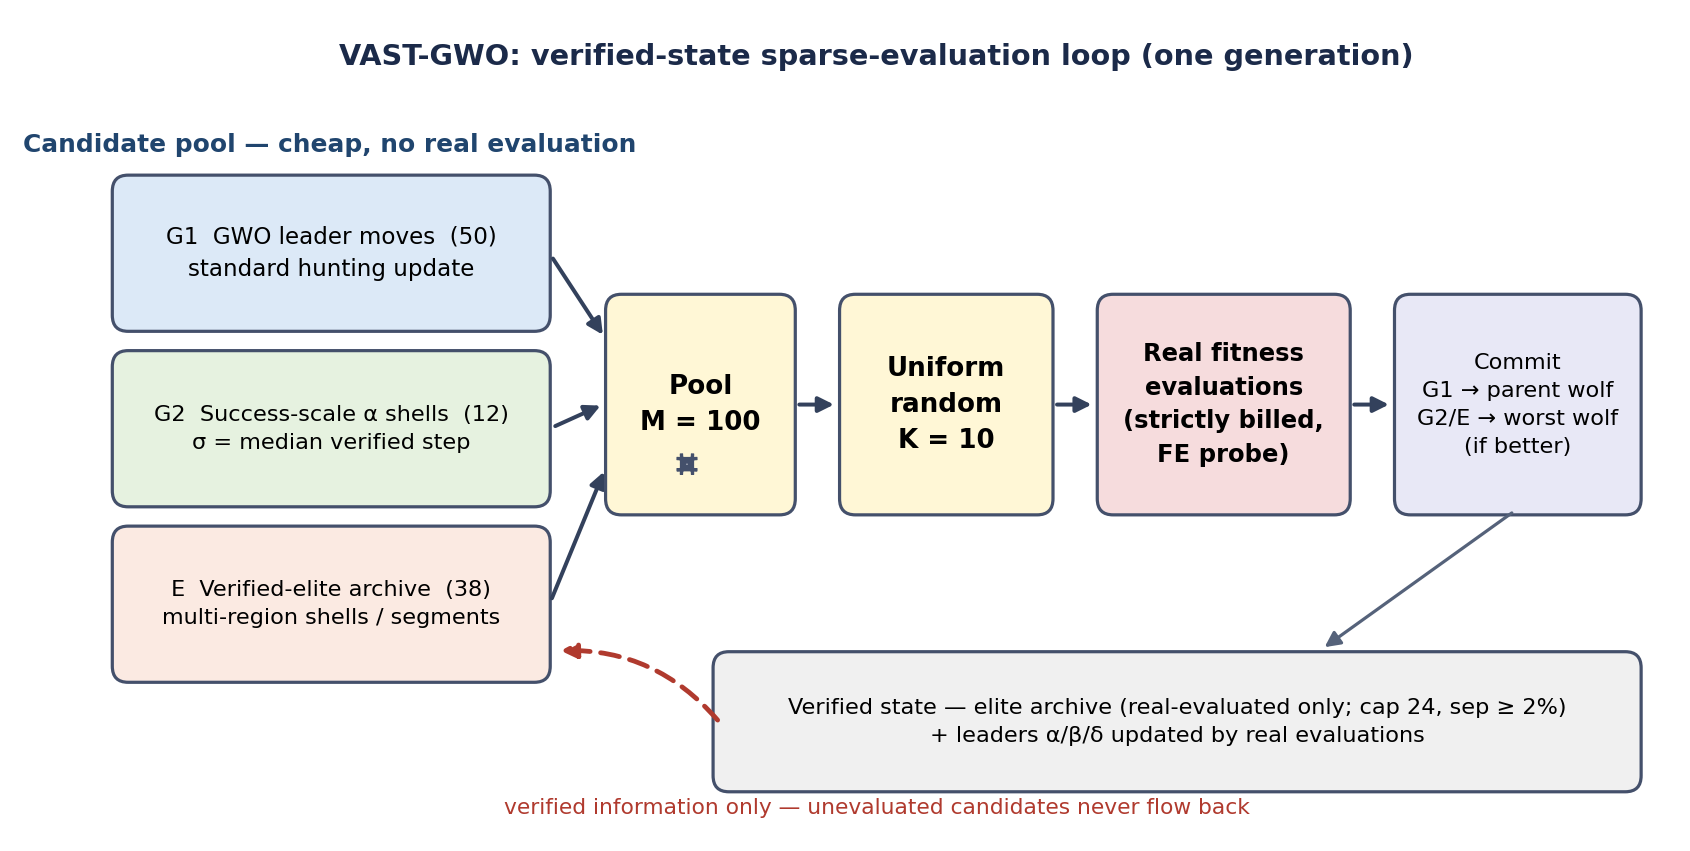
\includegraphics[width=0.92\linewidth]{figures/fig1_framework.png}
\caption{One generation of \method{}. A pool of 100 cheap candidates is
generated from three routes; only $K=10$ uniformly sampled candidates receive
a real (billed) evaluation, and only verified information flows back into the
leaders and the archive.}
\label{fig:framework}
\end{figure}

The three routes are complementary by design. Route G1 preserves the classical
hunting behaviour and moves the wolves themselves. Route G2 refines the
incumbent leader with a step scale that adapts to the geometry of recent
successful moves. Route E generates candidates from a verified multi-region
archive, providing both exploitation of verified basins (single-centre shells)
and interpolation between basins (two-centre segments). The allocation of
slots across the three routes ($50/12/38$) and the evaluated subset size
($K=10$) were fixed by a pre-registered development scan on development seeds
and functions before any formal run was executed
(Sections~\ref{sec:protocol}--\ref{sec:ablation}).

\subsection{Candidate generation routes}
\paragraph{G1: GWO leader moves (50 candidates).} For each wolf $i$ the
standard aggregation of the three leader-attracted positions is formed,
\begin{equation}
X_i^{G1}=\frac{1}{3}\sum_{k\in\{\alpha,\beta,\delta\}}
\left(X_k - A_k \odot \left| C_k \odot X_k - X_i \right|\right),
\end{equation}
with $A_k=2a\,r_1-a$ and $C_k=2r_2$, where $r_1,r_2\sim U(0,1)^D$ are drawn
per dimension and the convergence factor
\begin{equation}
a=2-2\,\mathrm{FE}/\mathrm{FE}_{\max}
\end{equation}
is driven by the true evaluation count rather than by an iteration counter.
This route preserves the classical exploration--exploitation schedule.

\paragraph{G2: success-scale alpha shells (12 candidates).} Local refinement is
generated in shells around the incumbent alpha wolf,
\begin{equation}
X^{G2}=X_\alpha+\sigma\odot(2u-1),\qquad u\sim U(0,1)^D,
\end{equation}
where the shell scale adapts to the observed geometry of successful moves,
\begin{equation}
\sigma=L\sqrt{3/D},\qquad
L=\max\!\left(\operatorname{median}(\sS_{25}),\;0.01\,d_{\mathrm{diag}}\right).
\label{eq:sigma}
\end{equation}
Here $\sS_{25}$ is the set of the 25 most recent \emph{verified} successful
step lengths (the Euclidean distance of an accepted move), $d_{\mathrm{diag}}$
is the diagonal of the search space, and $\sqrt{3/D}$ converts the
per-dimension half-width into an isotropic shell whose expected Euclidean
radius equals $L$. When fewer than five successful steps are available---only
at the start of a run---$L$ is initialised to $0.05\,d_{\mathrm{diag}}$. The
scale therefore follows the measured geometry of moves that worked instead of
a fixed schedule.

\paragraph{E: verified elite archive (38 candidates).} The archive stores up
to 24 real-evaluated solutions under two rules: a candidate may enter only if
it improves the worst archived objective value, and archived solutions are
kept separated by at least $2\%$ of $d_{\mathrm{diag}}$. If an evaluated
position is not separated from its nearest neighbour but is better than it,
the neighbour is replaced instead. Each archived centre carries a
\emph{credit} that counts how often it has contributed to an accepted
candidate. Nineteen of the 38 archive candidates are single-centre shells. A
centre $c$ is drawn with probability proportional to $1+\mathrm{credit}(c)$,
and the candidate is placed on a modulated shell,
\begin{equation}
X^{E_1}=c+\sigma\,(0.5+v)\odot(2u-1),\qquad v\sim U(0,1),
\end{equation}
so the shell radius varies in $[0.5\sigma,1.5\sigma]$ around the centre. The
remaining nineteen are two-centre segments between distinct archived centres
$c_1,c_2$,
\begin{equation}
X^{E_2}=c_1+\lambda\,(c_2-c_1)+0.25\,\sigma\odot(2u-1),
\qquad \lambda\sim U(0.15,0.85),
\label{eq:segment}
\end{equation}
which interpolate between verified basins. Because archived centres are
separated by construction, this route proposes candidates in several distinct
regions of the search space at the same time---the property that
Section~\ref{sec:ablation} identifies as the source of the method's
advantage.

\subsection{Sparse allocation and commit rules}
The $K=10$ evaluated candidates are drawn uniformly at random from the pool
without replacement. This keeps the allocation free of additional
hyperparameters and, as Section~\ref{sec:ablation} shows, is not improved upon
by screening, quota or learning-based alternatives. Commits follow the origin
of the candidate:
\begin{itemize}
\item an evaluated G1 candidate replaces its parent wolf if it improves that
parent's objective value;
\item an evaluated G2 or E candidate replaces the current worst wolf if it is
strictly better than that wolf;
\item every accepted move is appended to the verified-step record that drives
$\sigma$;
\item the archive and the leaders $\alpha,\beta,\delta$ are updated
exclusively from real-evaluated results.
\end{itemize}
All candidates are clamped to the search box before evaluation. Clamping is
the only boundary handling used; no reflection, re-sampling or repair is
applied, so the number of real evaluations consumed per generation is exactly
$K$ regardless of the geometry of the search space.

\begin{algorithm}[t]
\caption{\method{} (one run)}
\label{alg:vast}
\begin{algorithmic}[1]
\State initialize $N$ wolves by real evaluation; set
$\alpha,\beta,\delta$ and $\arc\!\leftarrow\!\emptyset$;
$\mathrm{FE}\!\leftarrow\!N$
\While{$\mathrm{FE}<\mathrm{FE}_{\max}$}
  \State build pool: 50 G1 moves, 12 G2 shells with scale
  $\sigma$ from Eq.~\eqref{eq:sigma}, 38 archive candidates
  \State sample $K=10$ candidates uniformly without replacement
  \For{each sampled candidate $x$}
     \State $f(x)\leftarrow$ real evaluation; $\mathrm{FE}\!\mathrel{+}\!=\!1$
     \State commit $x$ according to its route (parent or worst wolf, if
     better)
     \State update verified-step record, archive and
     $\alpha,\beta,\delta$ from verified results only
  \EndFor
\EndWhile
\State \Return best verified solution
\end{algorithmic}
\end{algorithm}

\subsection{Archive maintenance}
Algorithm~\ref{alg:archive} states the archive update and credit rule
explicitly, because the ablation in Section~\ref{sec:ablation} manipulates
this rule. The update is applied to every real-evaluated candidate, including
those that do not replace a wolf: the archive therefore accumulates the best
verified information of the run rather than only the winners of the current
generation. When the archive is full, an improving candidate that is
sufficiently separated from the stored solutions replaces the worst stored
solution; a candidate that is better than its nearest neighbour but too close
to it replaces that neighbour. The cold-start case is handled by an explicit
fallback: while the archive is empty, the archive slots are filled by
$\alpha$-centred shells, so the pool composition remains constant.

\begin{algorithm}[t]
\caption{Archive update (applied to every verified candidate $x$, value $v$)}
\label{alg:archive}
\begin{algorithmic}[1]
\If{$\arc=\emptyset$}
   \State $\arc\leftarrow\{x\}$
\ElsIf{$v<\max$ value in $\arc$}
   \If{distance from $x$ to nearest archive centre
   $\ge 0.02\,d_{\mathrm{diag}}$}
      \State insert $x$; if $\arc$ is full, replace the entry with the
      worst value and reset its credit
   \ElsIf{$v<$ value of the nearest archive centre}
      \State replace that centre by $x$
   \EndIf
\EndIf
\State if $x$ came from route E and was accepted, increment the credit of its
parent centre
\end{algorithmic}
\end{algorithm}

\subsection{Complexity}
Per generation, \method{} constructs $M=100$ candidates at cost $O(MD)$,
selects $K=10$ of them, performs $K$ objective evaluations, and maintains the
archive at cost $O(|\arc|D)$ per evaluated candidate with $|\arc|\le 24$. The
arithmetic cost of the search machinery is therefore a few thousand scalar
operations per real evaluation at $D=50$---negligible when evaluations are
expensive, and measurable when they are cheap. The number of generations is
fixed by the budget at $(\mathrm{FE}_{\max}-N)/K=9995$, so a run constructs
$999{,}500$ candidates for $100{,}000$ evaluations, i.e.\ ten candidates per
evaluation, and the additional arithmetic cost is reported as wall-clock time
at equal budget in Section~\ref{sec:results}.
\section{Experimental protocol}
\label{sec:protocol}
\subsection{Benchmarks and budgets}
All optimization experiments use the CEC2017 real-parameter suite in its
official 29-function form (F1 and F3--F30; F2 is omitted as in the official
definition) at dimension $D=50$, with a search domain of $[-100,100]^D$ and a
budget of 100{,}000 true objective evaluations per run, initialization
included \citep{awad2016problem}. Every algorithm is run 30 times per function
on seeds 3001--3030. For a given (function, seed) pair all algorithms start
from the same initial population, and the initialization and search random
streams are kept separate so that sharing the initial population does not
couple the trajectories. Two additional operating points are used to test
whether the conclusions are tied to one configuration: $D=100$ with
100{,}000 evaluations and ten seeds, and a five-times smaller budget of
20{,}000 evaluations at $D=50$ with ten seeds.

The mechanism study in Section~\ref{sec:ablation} uses a disjoint,
out-of-sample seed block (3071--3100). All five ablation arms are executed in
the same batch with identical pools, identical evaluated subset sizes and
identical budgets, so that only the composition of the candidate pool differs.

\subsection{Evaluation auditing and parallel execution}
Every objective call passes through an independent probe that counts true
evaluations, maintains a bounded reservoir of evaluated positions for unbiased
novelty estimation, and never perturbs the algorithm's random streams. Each
run asserts that the probe count equals the budget exactly, so no method can
gain from uncounted evaluations, restarts or cached duplicates. Runs are
executed on MATLAB R2025b with exactly four parallel workers (local
parpool, no serial fallback); each run writes its result atomically
and batches are resumable, so an interrupted batch resumes at the run level
without changing the experimental unit. All timings reported below are in-run
wall-clock times of the search phase, measured identically for every method on
the same machine (8-core AMD Ryzen 7 8745H, 16 threads, 15.3\,GB RAM).

\subsection{Baselines}
Six baselines are compared. Four are established methods: standard GWO
\citep{mirjalili2014gwo}, the strong improved GWO (I-GWO) with
dimension-wise opposition-based initialization, nonlinear control parameter
and dynamic position update \citep{nadimi2021igwo}, classic inertia-weight PSO
\citep{kennedy1995pso,shi1998modified} and CLPSO \citep{liang2006clpso}. Two
are recent 2026 variants whose authors provide open code: HAGWO, a hierarchical
adversarial GWO used here in its author implementation \citep{su2026hagwo}, and
AOGWO, an adaptive oppositional GWO, also in its author implementation
\citep{khalid2026aogwo}. Table~\ref{tab:setup} lists the source of each
implementation and the configuration used under the common protocol. Each
port to the common framework was restricted to interface and accounting
levels---initial population supplied by the framework, scheduling variable
expressed as a fraction of true evaluations, and one billed evaluation per
distinct position---so the search behaviour of every baseline is that of its
published or author-released form.

\begin{table}[t]
\centering
\small
\caption{Baselines, sources and configuration under the common protocol
($N=50$, identical initial populations, 100{,}000 true evaluations).}
\label{tab:setup}
\resizebox{\linewidth}{!}{\begin{tabular}{p{1.7cm}p{5.4cm}p{7.9cm}}
\toprule
Method & Source of the implementation & Configuration under the common protocol \\
\midrule
GWO & Original formulation, reimplemented and audited against the published equations \citep{mirjalili2014gwo} & $N=50$; whole pack evaluated once per iteration; linearly decreasing $a$; canonical boundary clamping \\
I-GWO & Published improved GWO \citep{nadimi2021igwo} & $N=50$; dimension-wise opposition-based initialization, nonlinear control parameter and dynamic position update as published \\
HAGWO & Author MATLAB code (commit bdfda96), hierarchical adversarial GWO \citep{su2026hagwo} & $N=50$; dynamic three-layer division, elite refinement, L\'evy perturbation and adversarial escape retained; per-iteration fitness reused instead of re-evaluated \\
PSO & Classic inertia-weight particle swarm \citep{kennedy1995pso,shi1998modified} & $N=50$; $w$ decreasing linearly from 0.9 to 0.4; $c_1=c_2=2$; $v_{\max}=0.2\,(\mathrm{ub}-\mathrm{lb})$ \\
CLPSO & TEC2006 author code package \citep{liang2006clpso} & $N=50$; $P_c$ schedule, five-stagnation refresh, $c=1.49445$; out-of-range positions are not re-evaluated, as in the original code \\
AOGWO & Author MATLAB code (commit 4122cef), adaptive oppositional GWO \citep{khalid2026aogwo} & $N=50$; oppositional initialization, cosine-adaptive $a$, decaying jump rate with L\'evy perturbation and selective opposition retained; search domain adapted to $[-100,100]^D$ \\
\bottomrule
\end{tabular}
}
\end{table}

\subsection{Statistics}
For each baseline we report the mean rank over the 29 functions, the
function-level win--loss record, the median paired error ratio of \method{}
over the baseline, the pooled $p$ value of the paired Wilcoxon signed-rank test
on $\log_{10}$ errors over identical seeds, and the Holm-corrected per-function
significant wins and losses. The primary evidence is the per-function paired
comparison: for each function the 30 paired runs are tested with a two-sided
Wilcoxon signed-rank test on $\log_{10}$ errors, and the resulting $p$ values
are corrected across the 29 functions with the Holm procedure; the sign of the
median paired difference determines whether a significant result counts as a
win or a loss. Median paired error ratios below one favour \method.
Bootstrap 95\% confidence intervals for median $\log_{10}$ gains are obtained
by resampling the paired differences. Pooled tests over all function--seed
pairs are reported for completeness but are not used as primary evidence,
because those pairs are not independent. Effect sizes in the application study
are reported as rank-biserial correlations.

Development and formal evaluation were separated. Hyperparameters, slot
allocations and the evaluated subset size were selected during a
pre-registered development phase on development functions and seeds; the
configuration was then frozen, and the formal batches reported here were
executed once. All configurations---including those that failed---are retained
in the experiment registry. The method's frozen implementation is
hash-identified, and a sampling audit confirms bitwise agreement between the
frozen configuration and the implementation used in the ablation batches.

\section{Results}
\label{sec:results}
\subsection{Comparison with strong baselines}
Table~\ref{tab:main} reports the final seven-method comparison and
Fig.~\ref{fig:ranks} the corresponding mean ranks. \method{} attains the best
mean rank, 2.24, ahead of the strong improved GWO (2.28), the 2026 hierarchical
HAGWO (3.41), PSO (4.41), CLPSO (4.48), the 2026 adaptive oppositional AOGWO
(5.07) and standard GWO (6.10). Against standard GWO the result is decisive:
28 wins in 29 functions, a median error ratio of 0.525, and 24 significant
wins with no significant loss after Holm correction. Against HAGWO, PSO, CLPSO
and AOGWO the margins are also significant (median ratios 0.806, 0.652, 0.668
and 0.586; Holm $+19/-3$, $+19/-2$, $+20/-5$, $+21/-0$). Against I-GWO---the
strongest classical improvement---the comparison is a statistical tie on
pooled error (ratio 0.938, 17 wins to 12 losses, pooled $p=0.55$), with a
median paired gain of $+0.023$ decades (95\% CI $[0.011,0.032]$) and large
function-level swings in both directions. The precise claim that this table
supports is therefore: \method{} is the best-ranked method of the seven and is
significantly better than five of six baselines, including both recent GWO
variants, while reaching parity with the strongest classical improvement.

\begin{table}[t]
\centering
\small
\caption{Final seven-method comparison (CEC2017, $D=50$, 100{,}000 true
evaluations, 29 functions, 30 runs on identical seeds). ``Median ratio'' is
the median paired error ratio of \method{} over the baseline (below one favours
\method); W--L counts functions whose mean error is lower/higher; Holm counts
per-function significant wins/losses after Holm correction; time is the mean
wall-clock time per run.}
\label{tab:main}
\resizebox{\linewidth}{!}{\begin{tabular}{lrrrrrr}
\toprule
Method & Med.\ ratio & W--L & Holm $+/-$ & Pooled $p$ & Mean rank & Time (s)\\
\midrule
\textbf{VAST-GWO} & -- & -- & -- & -- & \textbf{2.24} & 5.93\\
I-GWO & 0.938 & 17-12 & $+12/-6$ & $0.55$ & 2.28 & 2.32\\
HAGWO & 0.806 & 22-7 & $+19/-3$ & $2.2\times10^{-36}$ & 3.41 & 3.41\\
PSO & 0.652 & 23-6 & $+19/-2$ & $5.8\times10^{-31}$ & 4.41 & 2.59\\
CLPSO & 0.668 & 21-8 & $+20/-5$ & $7.4\times10^{-27}$ & 4.48 & 2.41\\
AOGWO & 0.586 & 27-2 & $+21/-0$ & $1.3\times10^{-85}$ & 5.07 & 4.54\\
GWO & 0.525 & 28-1 & $+24/-0$ & $6.7\times10^{-103}$ & 6.10 & 3.63\\
\bottomrule
\end{tabular}
}
\end{table}

\begin{figure}[t]
\centering
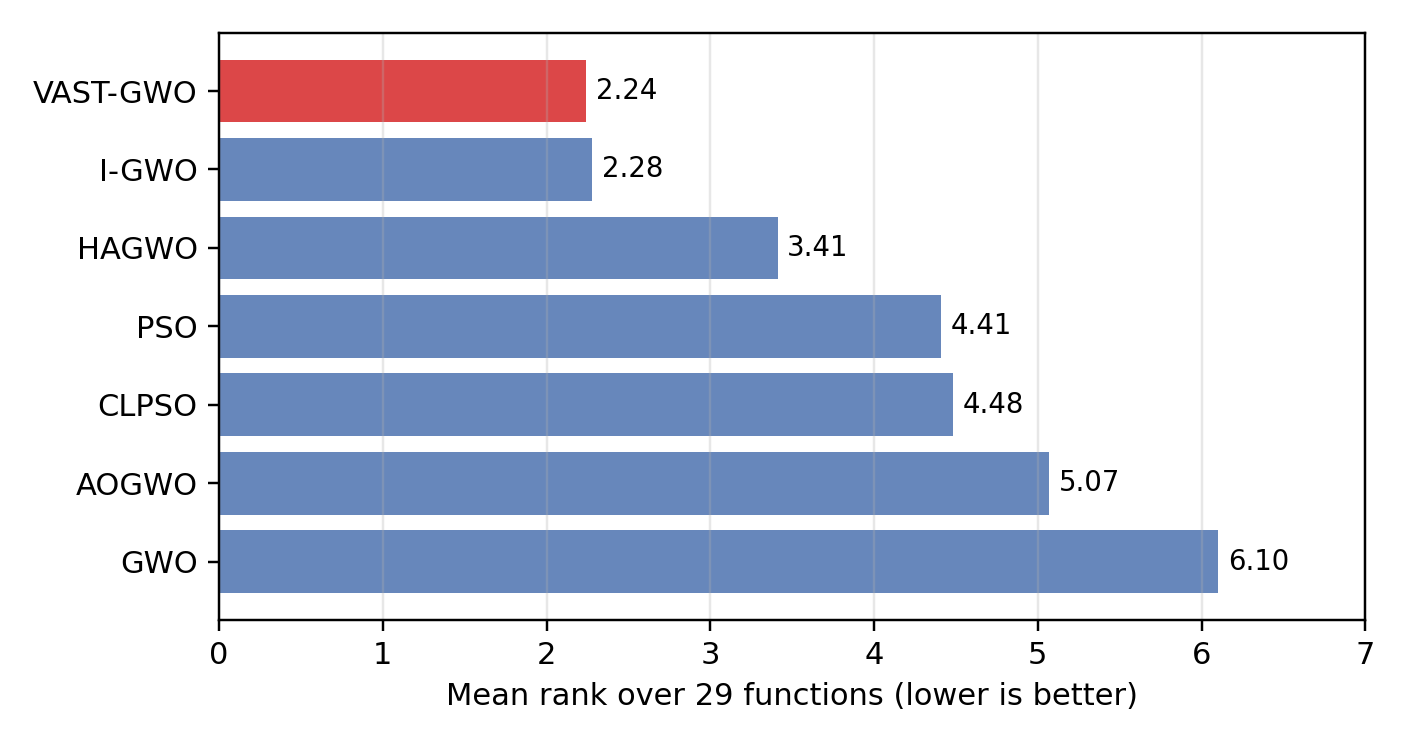
\includegraphics[width=0.75\linewidth]{figures/ranks7.png}
\caption{Mean rank over the 29 CEC2017 functions for the seven compared
methods ($D=50$, 100{,}000 true evaluations, 30 runs each).}
\label{fig:ranks}
\end{figure}

\subsection{Where the advantage lies: function families and per-function
structure}
The aggregate ranking hides a structured picture. \method{} holds the lowest
median error of the seven methods on 16 of the 29 functions: both unimodal
functions, four of the seven simple-multimodal functions, three of the ten
hybrid functions and seven of the ten composition functions. The largest
single-function margins are on F9, where the median error is 2.43 against
581.2 for the best competitor (a factor of 238), and on F1, where it is
$1.24\times10^{6}$ against $7.47\times10^{6}$ for the best competitor (a
factor of six) and roughly $5\times10^{3}$ better than standard GWO. Large but
narrower margins occur on F8, F20 and F21 (factors 1.46, 1.39 and 1.16).

Table~\ref{tab:family} and Fig.~\ref{fig:heatmap} break the comparison down by
benchmark family. Against the four weaker baselines and standard GWO the
advantage holds in every family, with ratios between 0.141 and 0.882; the
widest margins are on unimodal and simple-multimodal functions and the
narrowest on composition functions. Against I-GWO the picture is
function-dependent: \method{} leads on the unimodal, simple-multimodal and
composition families (median ratios 0.432, 0.796 and 0.932) while I-GWO
retains an advantage on hybrid functions (1.184). This is the honest
resolution of the parity reported above---the two strongest methods have
complementary family strengths---and it identifies hybrid functions as the
natural target for future mechanism work rather than as a deficit of the
comparison.

\begin{table}[t]
\centering
\small
\caption{Function-family median paired error ratios of \method{} over each
baseline (below one favours \method), with function-level win--loss counts in
parentheses. Families follow the CEC2017 classification: 2 unimodal, 7 simple
multimodal, 10 hybrid and 10 composition functions.}
\label{tab:family}
\resizebox{\linewidth}{!}{\begin{tabular}{lrrrr}
\toprule
Baseline & Unimodal & Simple multim. & Hybrid & Composition\\
\midrule
I-GWO & 0.432 (2-0) & 0.796 (4-3) & 1.184 (4-6) & 0.932 (7-3) \\
HAGWO & 0.227 (2-0) & 0.675 (4-3) & 0.769 (9-1) & 0.882 (7-3) \\
PSO & 0.187 (2-0) & 0.557 (5-2) & 0.653 (8-2) & 0.707 (8-2) \\
CLPSO & 0.144 (2-0) & 0.739 (4-3) & 0.662 (7-3) & 0.701 (8-2) \\
AOGWO & 0.148 (2-0) & 0.391 (6-1) & 0.513 (10-0) & 0.832 (9-1) \\
GWO & 0.141 (2-0) & 0.407 (6-1) & 0.407 (10-0) & 0.733 (10-0) \\
\bottomrule
\end{tabular}
}
\end{table}

\begin{figure}[t]
\centering
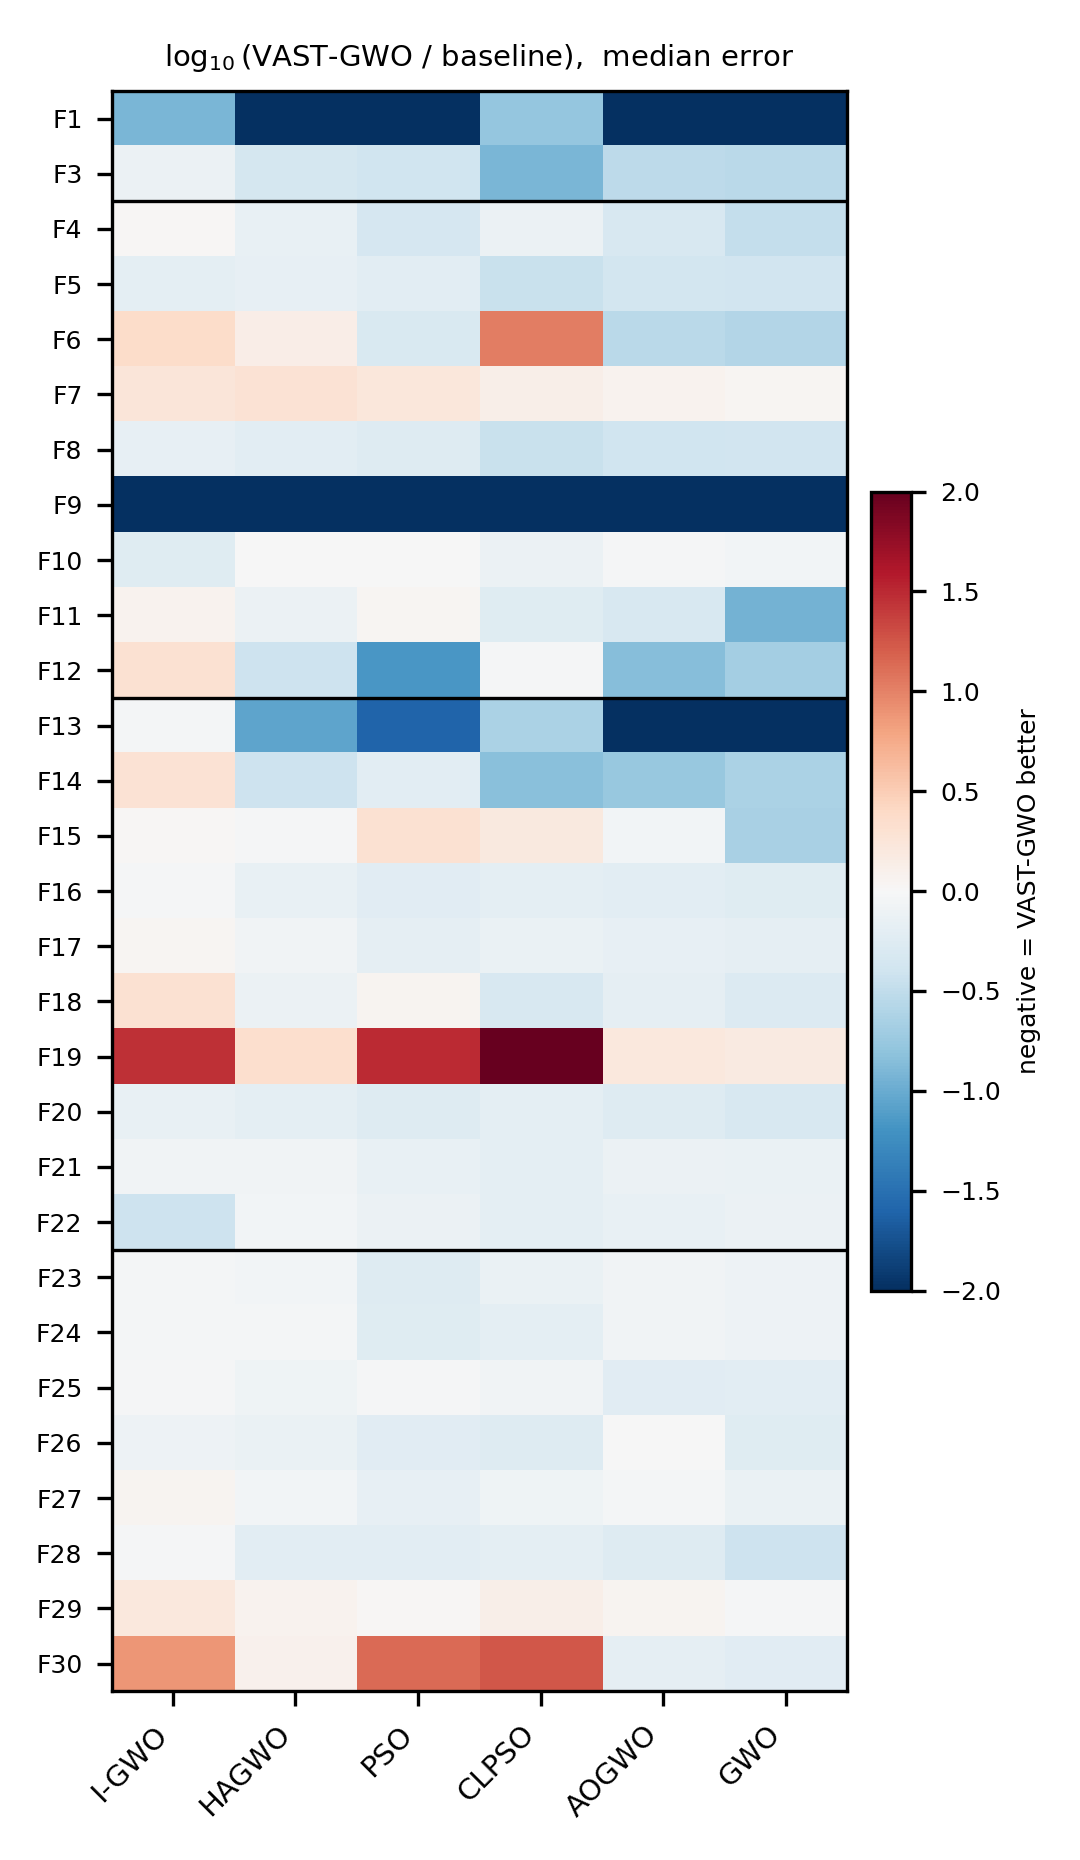
\includegraphics[width=0.62\linewidth]{figures/fig_heatmap.png}
\caption{Function-level median error ratios, $\log_{10}(\text{VAST-GWO} /
\text{baseline})$, for the six baselines. Blue indicates that \method{} has
the lower median error; values are clipped at $\pm 2$ decades. Horizontal
lines separate the unimodal, simple-multimodal, hybrid and composition
families.}
\label{fig:heatmap}
\end{figure}

\subsection{Convergence and exploration efficiency}
The advantage appears early and grows with the budget. At 10\%, 20\% and 50\%
of the evaluation budget the median error ratios against standard GWO are
0.802, 0.777 and 0.726, with 25, 26 and 27 of 29 functions respectively
better. Against the frozen development-phase reference (ANGWO) the ratios
are 0.732 and 0.768 at 10\% and 20\% of the budget, and on the
simple-multimodal subset (F4--F10) the ratio is 0.714. The same trajectories
explain how the budget is used: \method{} recovers from stagnation windows
more often than standard GWO (recovery probability 0.823 against 0.757) and
spends less of the budget inside long stagnation (long-stagnation share 0.813
against 0.844). On the exploration side, the useful-novelty rate---the share
of novel evaluations that are followed by a real improvement within a window
of $W=\max(50,1\%\,\mathrm{FE}_{\max})$ evaluations---is 0.00640 against
0.00347 for GWO and 0.00578 for ANGWO, and the novelty rate in
the final quarter of the budget is 0.712 against 0.588 for GWO. The
improving-evaluation rate in the final quarter is lower (0.00308 against
0.00481), which is consistent with a search that has already located its
productive regions and spends the remaining budget on novel exploration rather
than on incremental refinement. Table~\ref{tab:behaviour} reports all
behaviour metrics, and Fig.~\ref{fig:conv} shows representative convergence
curves.

\begin{table}[t]
\centering
\small
\caption{Behaviour metrics on the formal tier, computed from the stored
best-so-far traces with the definitions given in the text. S1 is the $K=50$
sparse variant, S3 a fixed quota policy and S5 a Q-learning policy
(Section~\ref{sec:ablation}); ANGWO is the frozen development-phase
reference.}
\label{tab:behaviour}
\resizebox{\linewidth}{!}{\begin{tabular}{lrrrrr}
\toprule
Method & Recovery prob. & Long-stag.\ share & Useful novelty & Novelty rate Q4 & Improving rate Q4 \\
\midrule
VAST-GWO ($K=10$) & \textbf{0.823} & \textbf{0.813} & \textbf{0.00640} & 0.712 & 0.00308 \\
S1 ($K=50$) & 0.816 & 0.812 & 0.00590 & 0.695 & 0.00266 \\
S3 (quota 25\%) & 0.808 & 0.821 & 0.00563 & 0.745 & 0.00272 \\
S5 (Q-learning) & 0.780 & 0.835 & 0.00629 & 0.716 & 0.00264 \\
ANGWO (frozen reference) & 0.768 & 0.831 & 0.00578 & 0.690 & 0.00447 \\
GWO & 0.757 & 0.844 & 0.00347 & 0.588 & 0.00481 \\
\bottomrule
\end{tabular}
}
\end{table}

\begin{figure}[t]
\centering
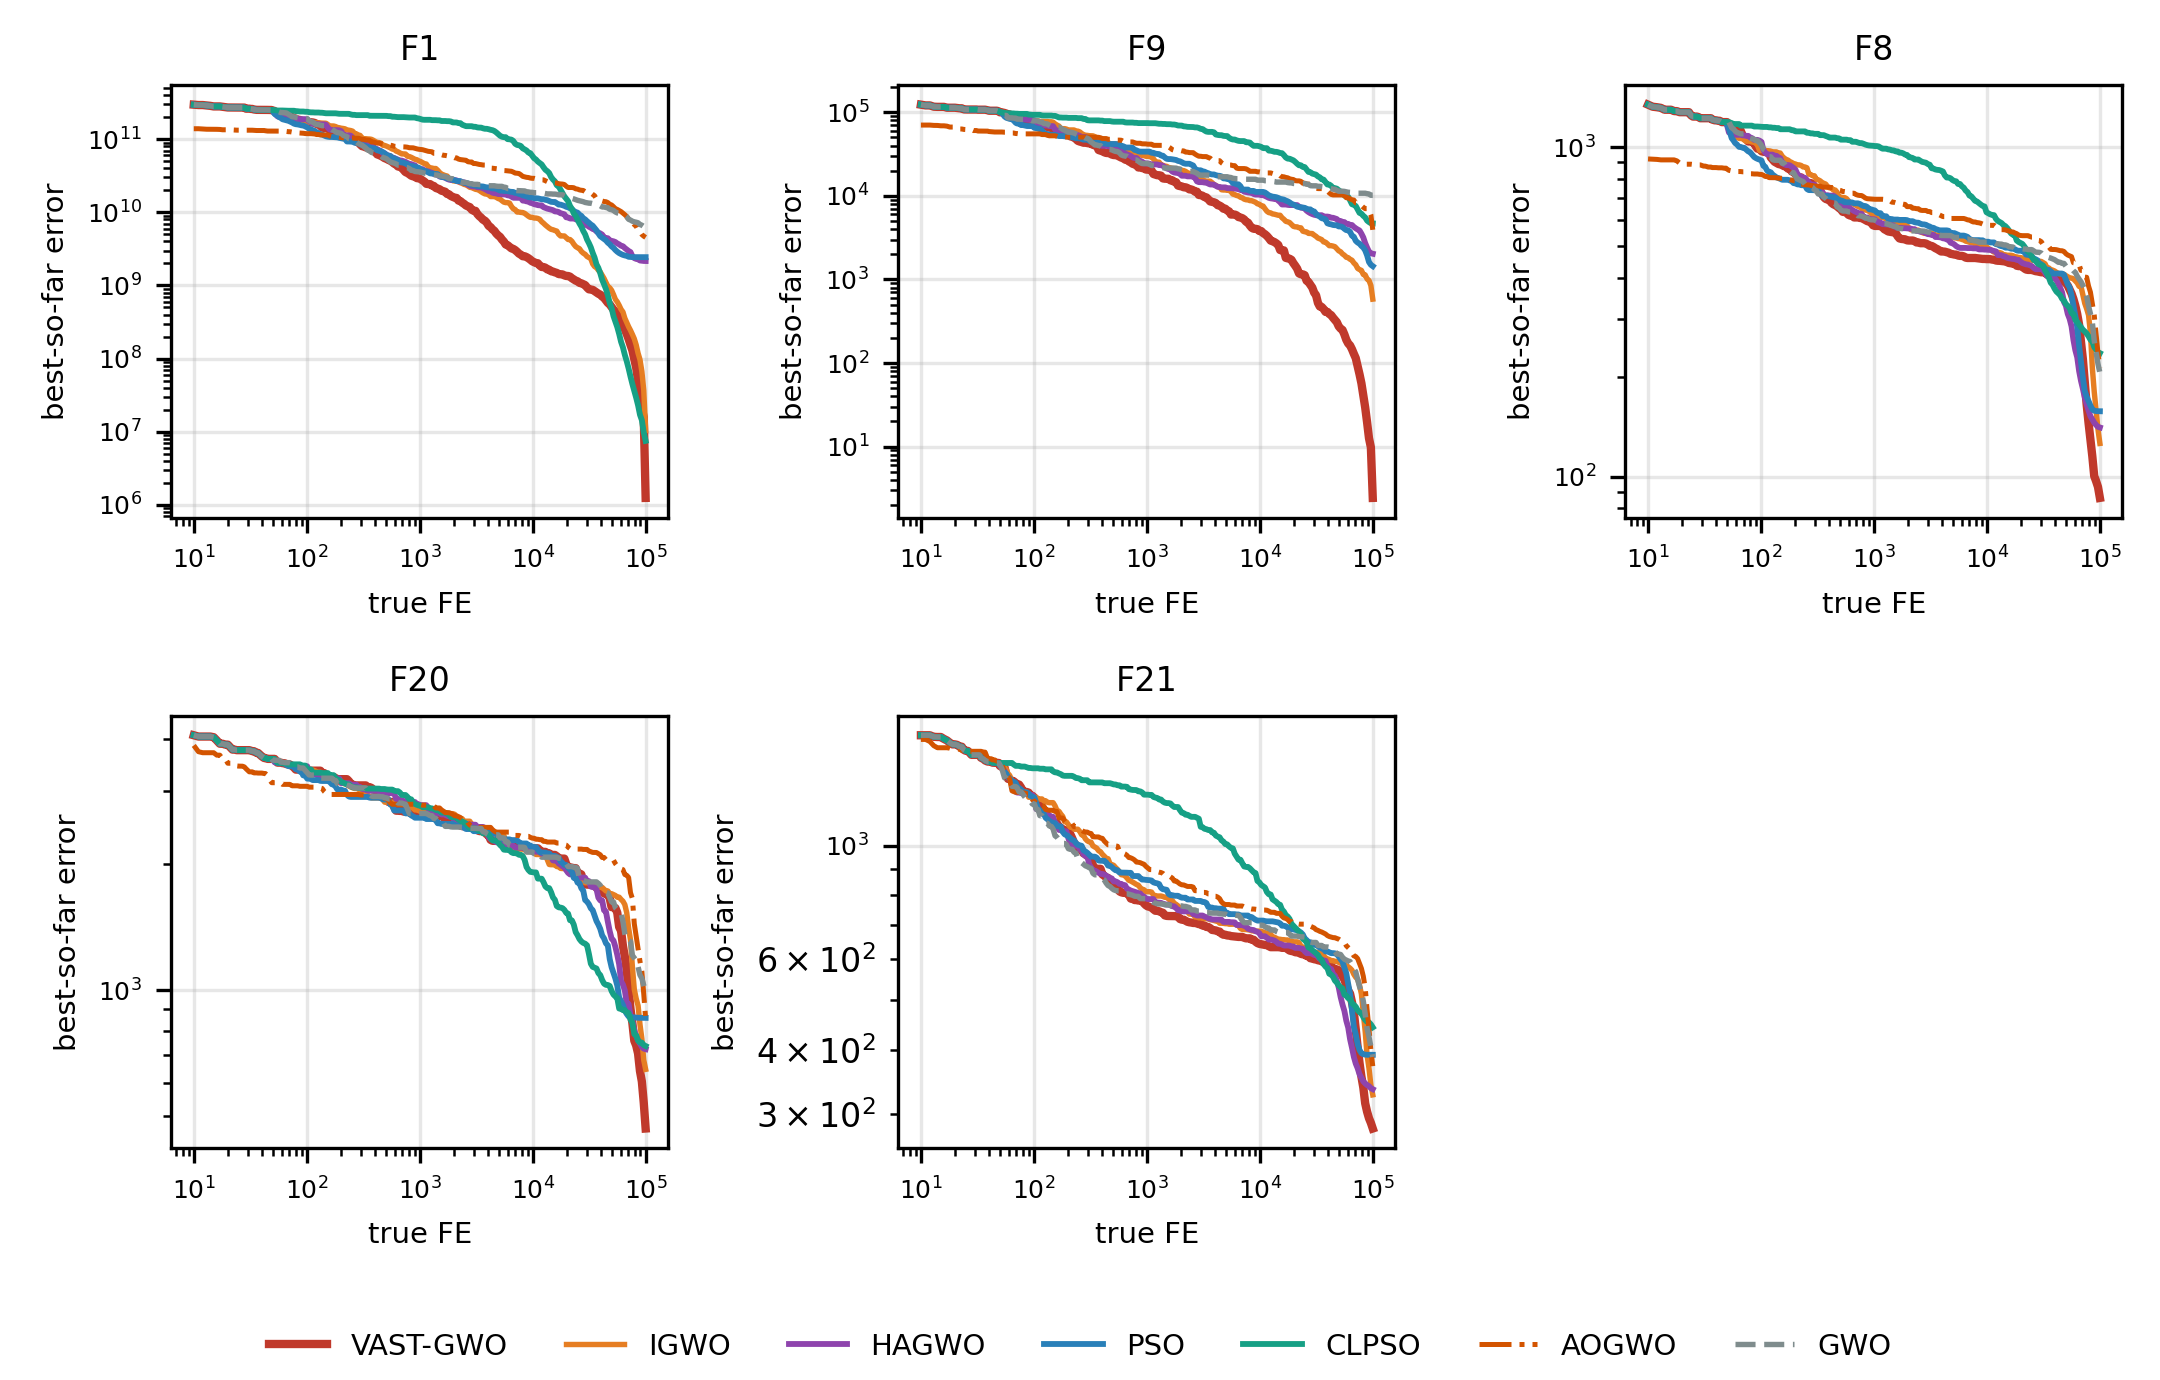
\includegraphics[width=\linewidth]{figures/fig_convergence.png}
\caption{Median best-so-far error of the seven compared methods over 30 runs on
five CEC2017 functions. The panels show the five functions on which
\method{} attains the largest final margin, one from each benchmark family plus
a second simple-multimodal function, so they illustrate the mechanism rather
than the average; the complete per-function picture is given by
Fig.~\ref{fig:heatmap} and Table~\ref{tab:main}.}
\label{fig:conv}
\end{figure}

\subsection{Additional operating points}
Table~\ref{tab:tiers} reports two further configurations. At $D=100$,
\method{} again ranks first (1.72 against 2.00, 2.33, 3.52 and 3.67 for the
compared variants), with a median ratio of 0.703 and 10 wins against 2 losses
(Holm $+5/-1$) against I-GWO on the twelve functions that both methods share,
and a ratio of 0.549 against a dense synchronous variant that evaluates every
individual. Under a budget five times smaller, \method{} also ranks first
(1.97), winning 24 of 29 functions against standard GWO (ratio 0.721), 24 of
29 against the frozen reference (0.807) and 24 of 29 against its dense variant
(0.678). The sparse-evaluation candidate pool therefore scales upward in
dimension and downward in budget, which is the regime relevant to engineering
problems where large budgets are unavailable.

\begin{table}[t]
\centering
\small
\caption{Additional operating points. Panel (a): $D=100$, 100{,}000
evaluations, 29 functions, ten seeds; the I-GWO ratio is computed on the twelve
functions shared with that implementation. Panel (b): 20{,}000 evaluations,
$D=50$, 29 functions, ten seeds. Ratios are relative to \method{} (below one
favours \method) with win--loss counts in parentheses.}
\label{tab:tiers}
\resizebox{\linewidth}{!}{\begin{tabular}{lrr}
\toprule
Method & Mean rank & Med.\ ratio vs VAST-GWO \\
\midrule
\multicolumn{3}{l}{\emph{(b) 20k FE, $D=50$, 29 functions, 10 seeds}}\\
VAST-GWO & \textbf{1.97} & -- \\
S1-K50 & 2.31 & 0.979 (17-12)\\
ANGWO & 3.10 & 0.807 (24-5)\\
B1-dense & 3.79 & 0.678 (24-5)\\
GWO & 3.83 & 0.721 (24-5)\\
\bottomrule
\end{tabular}
}
\end{table}

\subsection{Computational cost}
At equal budgets \method{} is the most expensive method in wall-clock terms:
5.93\,s per run at $D=50$ with 100{,}000 evaluations, against 3.63\,s for GWO,
3.41\,s for HAGWO, 2.59\,s for PSO, 2.41\,s for CLPSO, 2.32\,s for I-GWO and
4.54\,s for AOGWO; at $D=100$ the same budget costs 11.97\,s against 8.32\,s
and 7.83\,s for the compared dense and sparse variants. The overhead relative
to GWO is $1.6\times$ and originates in pool construction and archive
maintenance, both of which are arithmetic. In the regime \method{} targets---a
scarce number of expensive evaluations---this cost is negligible compared with
the objective, and it buys both the leading rank and the stagnation recovery
reported above. In the opposite regime, where evaluations are nearly free, the
runtime figures above allow the trade-off to be evaluated directly rather than
assumed.
\section{Ablation and mechanism analysis}
\label{sec:ablation}
\subsection{Equal-slot source ablation}
The ablation answers a single question by design: with the pool size, the
evaluated subset size, the budget and the acceptance rules held constant, which
compositions of the candidate pool produce the performance? Table~\ref{tab:abldesign}
lists the five arms. Arm A0 contains only standard GWO leader moves and
therefore measures what sparse evaluation alone achieves. A1 adds
leader-centred refinement, A2 adds the verified archive, A3 is the full method,
and A5 replaces the archive by a single alpha-centred sampler with identical
slot count, identical shell scale and identical acceptance rule, which isolates
the multi-region property of the archive from the mere presence of extra
perturbation.

\begin{table}[t]
\centering
\small
\caption{Equal-slot source ablation. All arms use $M=100$, $K=10$,
100{,}000 true evaluations and identical acceptance rules; only the
composition of the pool differs.}
\label{tab:abldesign}
\resizebox{\linewidth}{!}{\begin{tabular}{p{1.2cm}p{4.0cm}p{3.4cm}p{6.4cm}}
\toprule
Arm & Candidate pool (equal total $M=100$) & Mechanism under test & Rationale \\
\midrule
A0 & 100 GWO leader moves & Sparse evaluation alone & Isolates the effect of evaluating only $K$ of $M$ candidates \\
A1 & 50 GWO moves $+$ 50 $\alpha$-shells & Leader-centred refinement & Tests whether local refinement around $\alpha$ can replace multi-region memory \\
A2 & 50 GWO moves $+$ 50 archive candidates & Verified multi-region archive & Isolates the archive without the $\alpha$-shell route \\
A3 & 50 GWO moves $+$ 12 $\alpha$-shells $+$ 38 archive candidates & Full \method{} & Reference configuration \\
A5 & 50 GWO moves $+$ 12 $\alpha$-shells $+$ 38 single-centre draws around $\alpha$ & Archive replaced by a single centre with identical slots, scale and acceptance rule & Tests whether several regions, rather than extra perturbation, produce the gain \\
\bottomrule
\end{tabular}
}
\end{table}

Table~\ref{tab:abl} reports the outcome. Removing both auxiliary routes (A0)
degrades the method to 27 losses in 29 functions (median ratio 0.538, Holm
$+23/-0$): sparse evaluation by itself is not the source of the advantage.
Removing the archive while keeping the alpha shells (A1) still leaves the
method 25 functions behind the full version (0.812, Holm $+21/-1$). Keeping
the archive but removing the alpha shells (A2) leaves performance
statistically unchanged (0.994, 14--15, pooled $p=0.326$), so the alpha-shell
route is optional once the archive is present. Finally, replacing the archive
by a single-centre sampler with identical slots, scale and acceptance rule
(A5) collapses the method to 2 wins in 29 functions (1.407, Holm $+2/-23$).
The mean ranks over the five arms mirror the same ordering: A3 1.72, A2 1.79,
A5 3.34, A1 3.52, A0 4.62.

Two conclusions follow. First, the verified elite archive is the performance
engine of \method: A2, which contains only GWO moves and archive candidates,
is statistically indistinguishable from the full method while beating the
GWO-only pool 29--0. Second, it is the \emph{multi-region} character of the
archive that matters rather than the amount of additional perturbation: A5
uses the same number of extra candidates, the same shell scale and the same
acceptance rule, and differs from the full method only in drawing those
candidates from one centre instead of several, yet its performance falls by a
factor of 1.41. The source-level attribution in Fig.~\ref{fig:sources}
confirms the same picture at the level of accepted events: in a full run the
archive route produces on average 24{,}068 accepted improvements, against
11{,}325 for the GWO-move route and 4{,}742 for the alpha-shell route.

\begin{table}[t]
\centering
\small
\caption{Equal-slot candidate-source ablation (29 functions, 30 seeds
3071--3100, 100{,}000 true evaluations each). Ratios are relative to the full
configuration; Holm counts the significant wins/losses of the listed
comparison.}
\label{tab:abl}
\resizebox{\linewidth}{!}{\begin{tabular}{lrrrr}
\toprule
Comparison & Median ratio & W--L & Holm $+/-$ & Pooled $p$ \\
\midrule
A3 (full) vs A0 (GWO moves only) & 0.538 & 27--2 & $+23/-0$ & $7\times10^{-102}$ \\
A3 (full) vs A1 (G1$+$G2) & 0.812 & 25--4 & $+21/-1$ & $5\times10^{-60}$ \\
A3 (full) vs A2 (G1$+$E) & 0.994 & 14--15 & $+1/-0$ & 0.326 \\
A2 (G1$+$E) vs A0 & 0.510 & 29--0 & $+27/-0$ & $7\times10^{-117}$ \\
A5 (single centre) vs A3 (full) & 1.407 & 2--27 & $+2/-23$ & $1\times10^{-64}$ \\
\bottomrule
\end{tabular}
}
\end{table}

\begin{figure}[t]
\centering
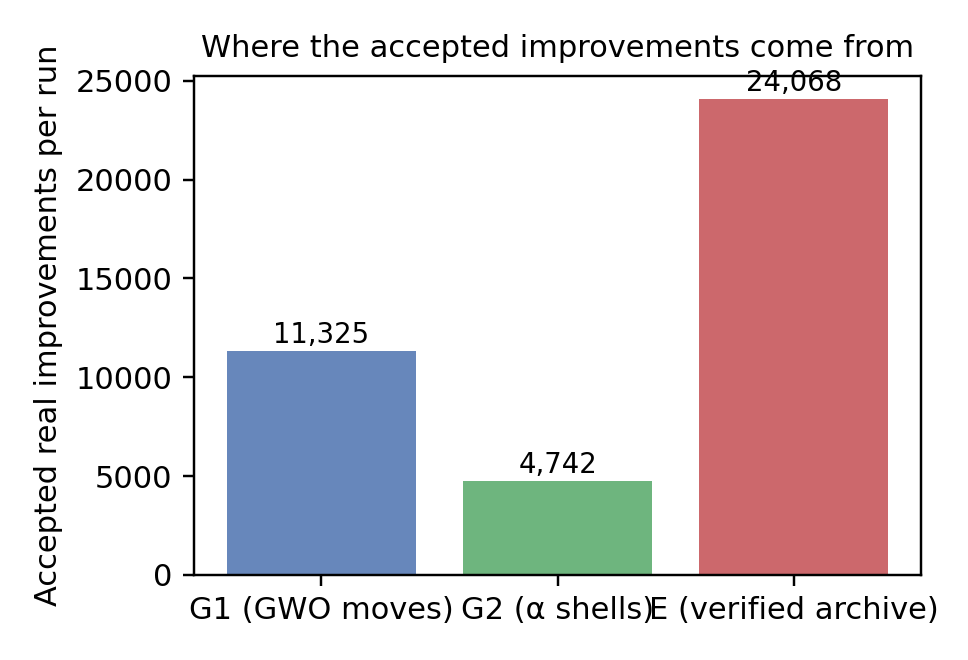
\includegraphics[width=0.70\linewidth]{figures/fig4_sources.png}
\caption{Accepted real improvements per run by candidate route, averaged over
the ablation batch. The verified archive route dominates; the alpha-shell
route is the smallest contributor, consistent with its optional role once the
archive is present.}
\label{fig:sources}
\end{figure}

\subsection{Design-space boundaries and rejected alternatives}
The same controlled protocol was used to test the natural alternatives to
uniform random allocation and to two popular enhancement strategies
(Table~\ref{tab:bound}). Every one of them was rejected by its pre-registered
criterion. Directed screening by proximity to the incumbent and by archive
credit is worse than uniform sampling (median ratio 1.394) because it starves
the GWO route of evaluations; informed stratified allocation (1.528),
pool-ratio allocation (1.255) and trend-informed allocation (1.348) are also
worse than the uniform draw; fixed exploration quotas of 0.25, 0.50 and 0.75
degrade performance (1.070, 1.064 and 1.672); and three Q-learning quota
schedulers---with zero, tuned and prior-initialised Q tables---never exceed the
best fixed policy (0.988, 1.024 and 1.130), although all of them beat random
quota perturbation (0.748--0.870). A stagnation-triggered radius boost
degrades final quality (1.204). Finally, steering moves along previously
successful directions improves the final error against the frozen
configuration (0.897, 21 wins in 29 functions), but an equal-magnitude
random-direction control reproduces the effect (0.988 between the two steering
variants, pooled $p=0.155$), and the gain appears only in the last 20\% of the
budget while wall-clock time rises by 17--25\%. The mechanism was therefore
rejected as an information-driven contribution and is not part of \method.

\begin{table}[t]
\centering
\small
\caption{Design-space boundary experiments. Each hypothesis was tested with a
matched control under the common protocol; ratios below one favour the control
variant and ratios above one favour the reference configuration.}
\label{tab:bound}
\resizebox{\linewidth}{!}{\begin{tabular}{p{4.6cm}p{4.2cm}p{2.6cm}p{4.0cm}}
\toprule
Hypothesis & Control & Median ratio & Verdict \\
\midrule
Screening the best-looking candidates beats random allocation & Directed screening by proximity to $\alpha$ and archive credit (S2) & 1.394 vs uniform & Rejected; it starves the GWO route of evaluations \\
Stratified or informed allocation beats a uniform draw & Informed-in-strata, pool-ratio and trend-informed allocation & 1.528 / 1.255 / 1.348 & Rejected \\
A fixed exploration quota manages the budget better than the pool share & Fixed quota at 0.25 / 0.50 / 0.75 & 1.070 / 1.064 / 1.672 & Rejected; raising the quota above the pool share is harmful \\
Reinforcement learning schedules the budget better than the best fixed policy & Three Q-learning quota schedulers (zero, tuned and prior-initialised) & 0.988--1.130 vs best fixed; 0.748--0.870 vs random quota & Rejected as a contribution; always at or below the best fixed policy \\
A stagnation-triggered radius boost restores progress & Shell radius multiplied by three after stagnation & 1.204 & Rejected \\
Reusing verified successful directions adds information beyond extra perturbation & Steering along the mean recent successful direction & 0.897 vs frozen; 0.988 vs equal-magnitude random directions ($p=0.155$) & Rejected; the random control reproduces the gain \\
\bottomrule
\end{tabular}
}
\end{table}

\subsection{Interpretation of the mechanism evidence}
Three statements are supported by the ablation and boundary results, and one
is not. Supported: (i) sparse evaluation alone is not sufficient---the
GWO-only pool loses 27 of 29 functions to the full method; (ii) verified
multi-region memory is the dominant source of the improvement---removing the
archive costs 25 functions, replacing it with a single centre costs 27, and
the archive route accounts for the majority of accepted improvements; (iii)
the allocation rule does not need to be learned or tuned---uniform sampling
dominates or matches every alternative tested, including three Q-learning
schedulers with matched controls. Not supported: alpha-centred local
refinement is not necessary once the archive exists, since A2 and A3 are
statistically indistinguishable. The implication is a design rule rather than
a mechanism stack: make the candidate pool contain verified information from
several regions, and keep the evaluation rule simple.

\section{Application: 3D UAV delivery path planning}
\label{sec:uav}
\subsection{Problem formulation}
The application is a three-dimensional UAV delivery problem with hard time
windows, built on real terrain data. Each instance contains 20 delivery
stations with individual time windows, a depot, three cylindrical threat zones
and three intermediate control points per flight leg. A candidate solution is
a decision vector of dimension
\begin{equation}
D=20+\underbrace{21\times3\times3}_{\text{21 legs, 3 control points, 3 offsets}}
=209 .
\end{equation}
The first 20 coordinates define the visiting order through their rank; the
remaining 189 coordinates define, for each leg, three control points by a
position ratio along the straight line from the current point to the next
target, a lateral offset and a height offset. The decoded trajectory is a
sequence of legs from the depot through all stations and back to the depot.

The objective combines total flight distance, waiting time and path
smoothness,
\begin{equation}
\label{eq:uavobj}
J=\sum_{\ell} d_\ell+0.05\sum_{\ell} w_\ell+2\sum_{\ell} s_\ell ,
\end{equation}
where $d_\ell$ is the length of leg $\ell$, $w_\ell$ is the waiting time
accumulated before a station's ready time, and $s_\ell$ penalises turn and
pitch changes. Hard constraints are imposed on terrain clearance, threat-zone
avoidance, maximum altitude, climb and turn limits, the delivery time windows
and the return to the depot, with penalty terms that keep infeasible solutions
strictly behind feasible ones. Table~\ref{tab:uavmodel} lists the model
parameters; the five scenarios use real Copernicus GLO-90 terrain tiles with
distinct morphology (ridge, peaks, mountain, hills and plateau) and were frozen
before the formal runs.

\begin{table}[t]
\centering
\small
\caption{Parameters of the 3D UAV delivery benchmark (benchmark-v1). The
benchmark is a normalized simulation derived from real terrain data, not a
flight test.}
\label{tab:uavmodel}
\resizebox{\linewidth}{!}{\begin{tabular}{p{4.4cm}p{3.6cm}p{7.0cm}}
\toprule
Quantity & Value & Role in the model \\
\midrule
Decision vector & 209 dimensions & 20 ranking values for the visiting order $+$ 189 control offsets (21 legs $\times$ 3 control points $\times$ 3 offsets) \\
Map extent & $100\times100$ units & Horizontal extent of each terrain tile; depot at $(40,50)$ \\
Terrain & Copernicus GLO-90, five tiles & Ridge, peaks, mountain, hills and plateau; bilinear interpolation on a $51\times51$ grid \\
Delivery points & 20 per map & Fixed station coordinates; five-digit hard time windows per station \\
Cruise speed & 10 units per time unit & Converts leg length to arrival time \\
Service height & 16 m above ground & Station altitude; depot altitude follows the terrain \\
Terrain clearance & 4 m & Minimum vertical separation between route and terrain along each leg \\
Threat zones & 3 cylinders per map & Radius plus 2 m safety margin; vertical extent from terrain base to a specified ceiling \\
Operating ceiling & 42 m & Maximum flight altitude \\
Climb / turn limits & $35^\circ$ / $120^\circ$ & Maximum flight-path angle and heading change within a leg \\
Objective weights & 1 / 0.05 / 2 & Distance, waiting time and smoothness terms in Eq.~\eqref{eq:uavobj} \\
Penalties & $10^5+10^3\Delta t$ / $10^5+10^4\Delta g$ & Time-window lateness and geometric violations, respectively \\
\bottomrule
\end{tabular}
}
\end{table}

\subsection{Protocol and metrics}
All six methods run with $N=50$ and 30{,}000 true evaluations per run,
initialization included, on 30 repetitions for each of the five scenarios,
giving $6\times5\times30=900$ independent runs. Each method starts from the
same initial population for a given (map, repetition), the search random
stream is offset identically, and every run is verified after the search with
the full evaluator outside the billed budget. Four quantities are reported
because they answer different engineering questions: the final feasibility
rate; the time to the first feasible route, summarised by the restricted mean
survival time (RMST) under a 30{,}000-evaluation censoring horizon, in which
every run enters the statistic; the cumulative feasibility at 2k, 5k, 10k, 20k
and 30k evaluations; and the final route cost on paired runs in which both
methods were feasible. Final feasibility is compared with McNemar tests,
route cost with paired Wilcoxon tests and rank-biserial effect sizes, and time
to feasibility with a censoring-aware ordered test on the checkpoint at which
feasibility was first reached.

\subsection{Results}
\method{} is the only method that finds a feasible route in every one of its
150 runs; the runner-up reliability is 97.3\% (I-GWO and HAGWO), followed by
PSO (95.3\%), GWO (94.0\%) and CLPSO (61.3\%). It also attains the smallest
RMST, 7{,}062 evaluations (95\% CI 6{,}449--7{,}731), ahead of HAGWO (8{,}133),
PSO (8{,}138), GWO (10{,}936), I-GWO (12{,}270) and CLPSO (24{,}427). The
cumulative feasibility curves show where the advantage appears: at 10{,}000
evaluations \method{} has already reached 82.0\% feasibility, against 76.0\%
for HAGWO and 74.0\% for PSO, and at 20{,}000 evaluations it reaches 100\%
while every other method is still between 26.7\% and 97.3\%. Table~\ref{tab:uav}
summarises reliability and quality, Figs.~\ref{fig:uavfeas}--\ref{fig:uavroutes}
show the behaviour in detail, and Table~\ref{tab:uavmaps} reports the per-map
feasibility rates, where \method{} achieves 100\% on all five terrains.

Final route quality favours \method{} against every baseline. Over the pairs
in which both methods were feasible, the median paired cost ratios are 0.939
against GWO, 0.898 against I-GWO, 0.967 against HAGWO, 0.843 against PSO and
0.631 against CLPSO, and all five remain significant after Holm correction
($p$ from $3.3\times10^{-16}$ to $0.0458$, rank-biserial 0.19--1.00). The
censoring-aware ordered test is significant against GWO, I-GWO, HAGWO and
CLPSO; the exception is PSO ($p=0.598$), which finds feasible routes earlier
in the first few thousand evaluations (median 5{,}357 against 6{,}314 in
successful runs) and then stalls: its final routes are markedly worse (median
cost 766.4 against 667.4) and it misses feasibility in seven runs. HAGWO's
marginal median cost (663.4) is slightly below that of \method{} (667.4) when
each method's own successful runs are considered separately; on the 146 runs
where both methods succeed, \method{} is significantly better (ratio 0.967,
Holm $p=0.0458$). McNemar tests on final feasibility are significant against
GWO ($p=0.016$), PSO ($p=0.047$) and CLPSO ($p<10^{-16}$) after Holm
correction, while the reliability difference against I-GWO and HAGWO---both of
which fail four runs---is not significant on four discordant pairs.

\begin{table}[t]
\centering
\small
\caption{3D UAV delivery application (150 runs per method: five maps, 30
repetitions). Feasibility is the share of runs that found a feasible route
within 30{,}000 evaluations; RMST is the restricted mean time to first
feasibility under a 30{,}000-evaluation censoring horizon, so all runs enter
the statistic; the first-feasible median is conditional on successful runs and
is shown for reference; cost is the median final route cost over feasible runs
(lower is better).}
\label{tab:uav}
\resizebox{\linewidth}{!}{\begin{tabular}{rrrrrr}
\toprule
Method & Feasible (\%) & RMST & RMST 95\% CI & First feasible$^{\dagger}$ & Cost$^{\ddagger}$ \\
\midrule
\method{} & \textbf{100.0} & \textbf{7062} & [6449, 7731] & 6314 & 667.4 \\
GWO & 94.0 & 10936 & [9941, 11983] & 8920 & 699.8 \\
I-GWO & 97.3 & 12270 & [11374, 13179] & 11152 & 724.7 \\
HAGWO & 97.3 & 8133 & [7355, 8950] & 7432 & 663.4 \\
PSO & 95.3 & 8138 & [7058, 9324] & 5357 & 766.4 \\
CLPSO & 61.3 & 24427 & [23312, 25383] & 21330 & 1015.4 \\
\bottomrule
\end{tabular}
}
\end{table}

\begin{table}[t]
\centering
\small
\caption{Per-map feasibility (\% of 30 runs) on the five terrain scenarios.}
\label{tab:uavmaps}
\resizebox{\linewidth}{!}{\begin{tabular}{lrrrrr}
\toprule
Method & Hills & Mountain & Peaks & Plateau & Ridge \\
\midrule
\method{} & \textbf{100} & \textbf{100} & \textbf{100} & \textbf{100} & \textbf{100} \\
GWO & 96.7 & 83.3 & 100 & 90.0 & 100 \\
I-GWO & 100 & 86.7 & 100 & 100 & 100 \\
HAGWO & 96.7 & 93.3 & 100 & 96.7 & 100 \\
PSO & 100 & 83.3 & 100 & 96.7 & 96.7 \\
CLPSO & 56.7 & 36.7 & 80.0 & 60.0 & 73.3 \\
\bottomrule
\end{tabular}
}
\end{table}

\begin{figure}[t]
\centering
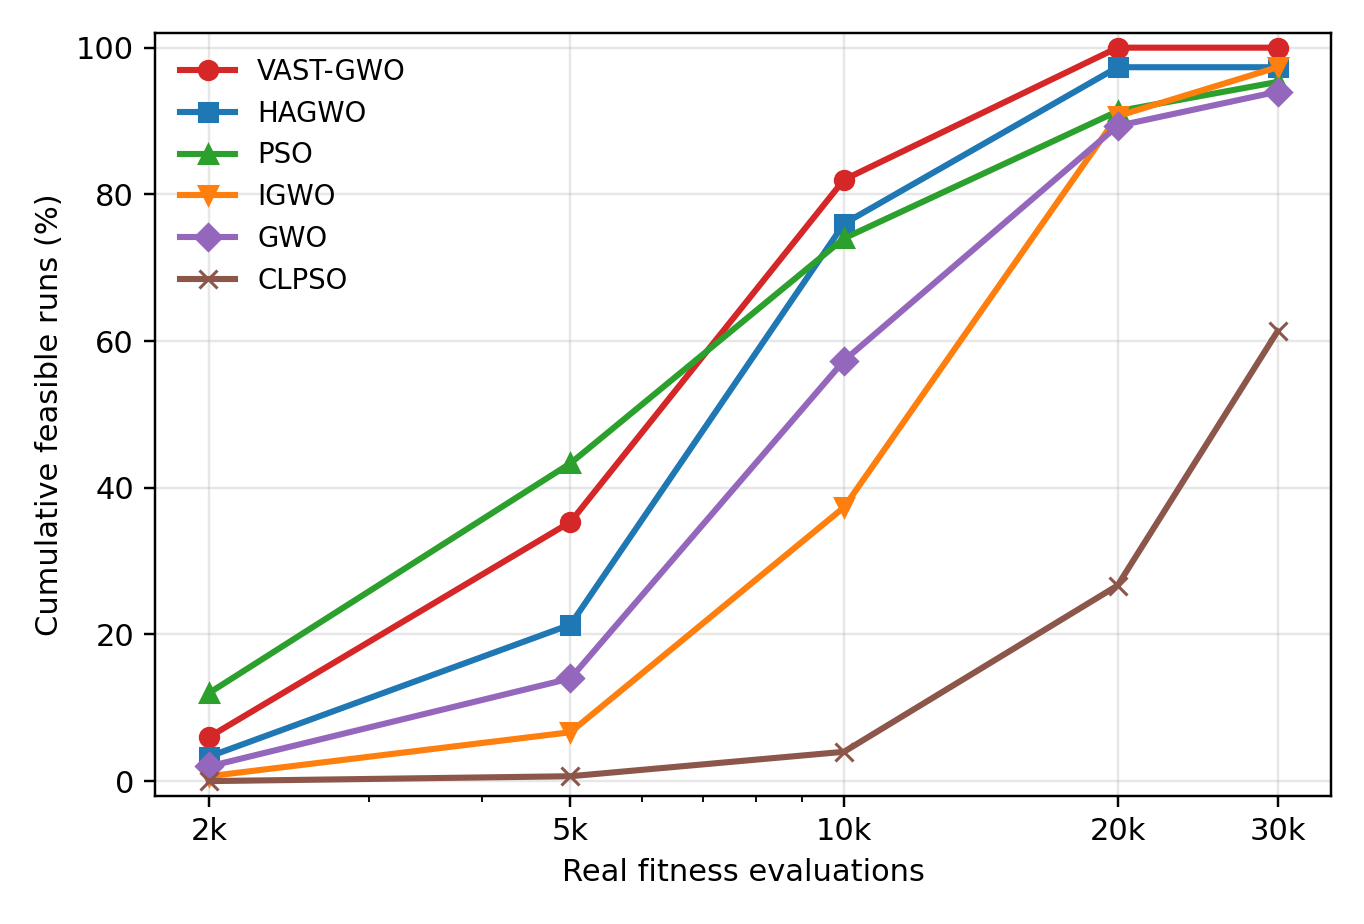
\includegraphics[width=0.92\linewidth]{figures/uav_feasibility_curve.png}
\caption{Cumulative feasible runs versus real evaluations on the five
DEM-based delivery scenarios (150 runs per method). Checkpoints are early
observations within the single 30k protocol.}
\label{fig:uavfeas}
\end{figure}

\begin{figure}[t]
\centering
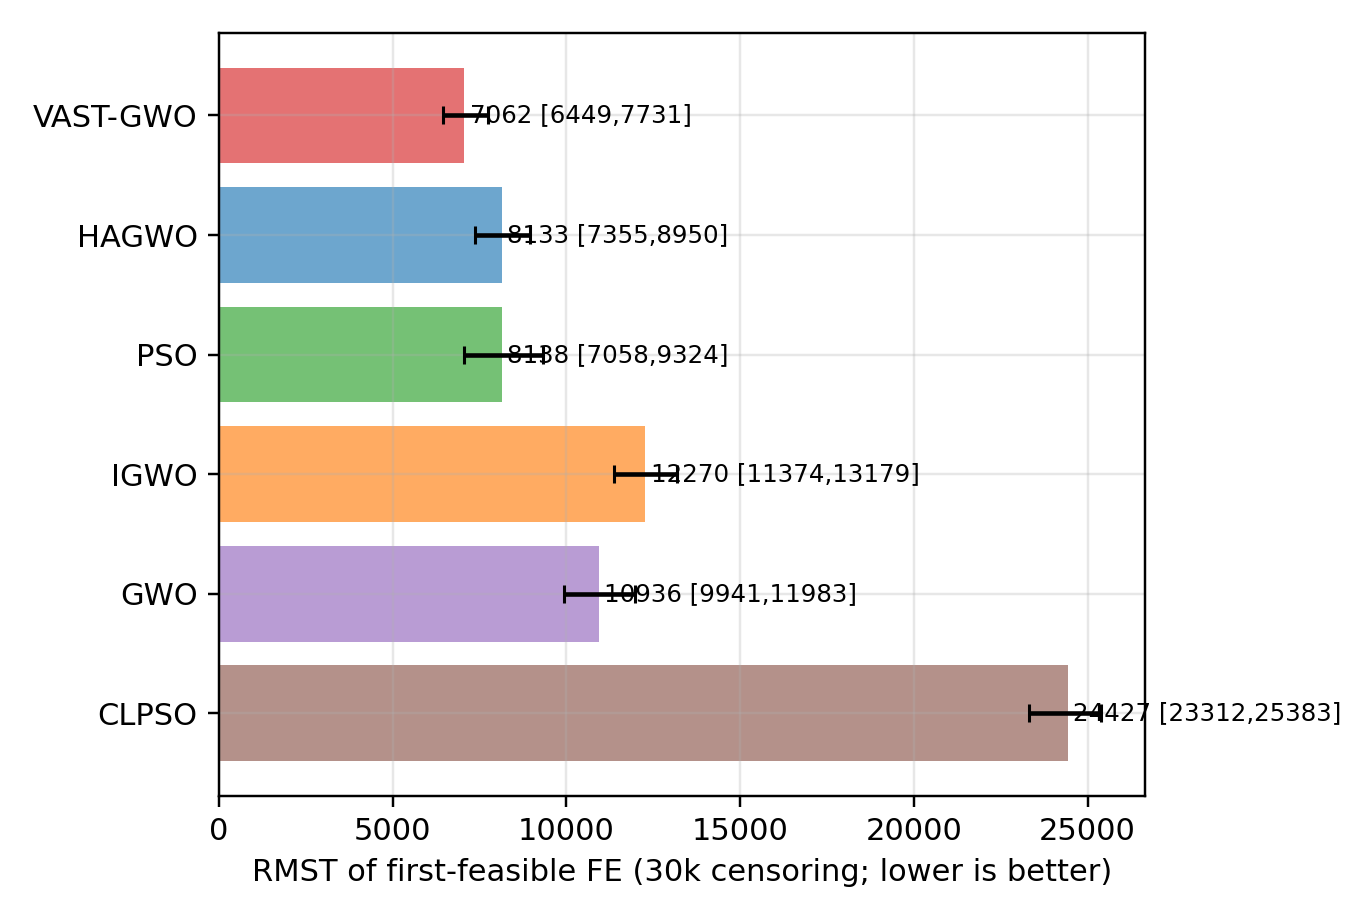
\includegraphics[width=0.92\linewidth]{figures/uav_rmst_bar.png}
\caption{Censored mean time to first feasible route (RMST, 30k horizon,
bootstrap 95\% confidence intervals). Every run enters the statistic.}
\label{fig:uavrmst}
\end{figure}

\begin{figure}[t]
\centering
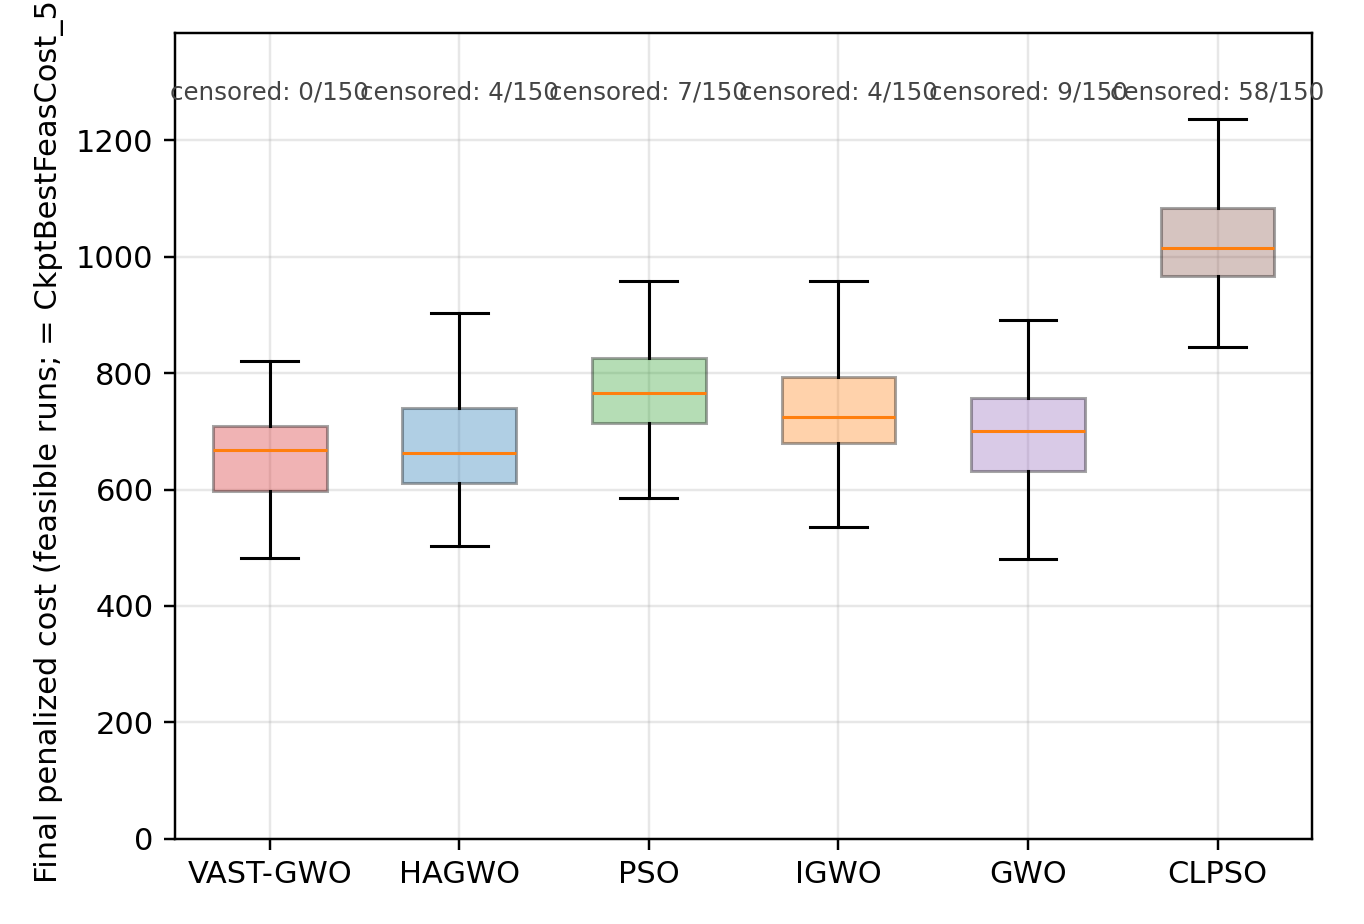
\includegraphics[width=0.92\linewidth]{figures/uav_final_cost_box.png}
\caption{Distribution of final feasible route cost per method over the five
scenarios and 30 repetitions.}
\label{fig:uavcost}
\end{figure}

\begin{figure}[t]
\centering
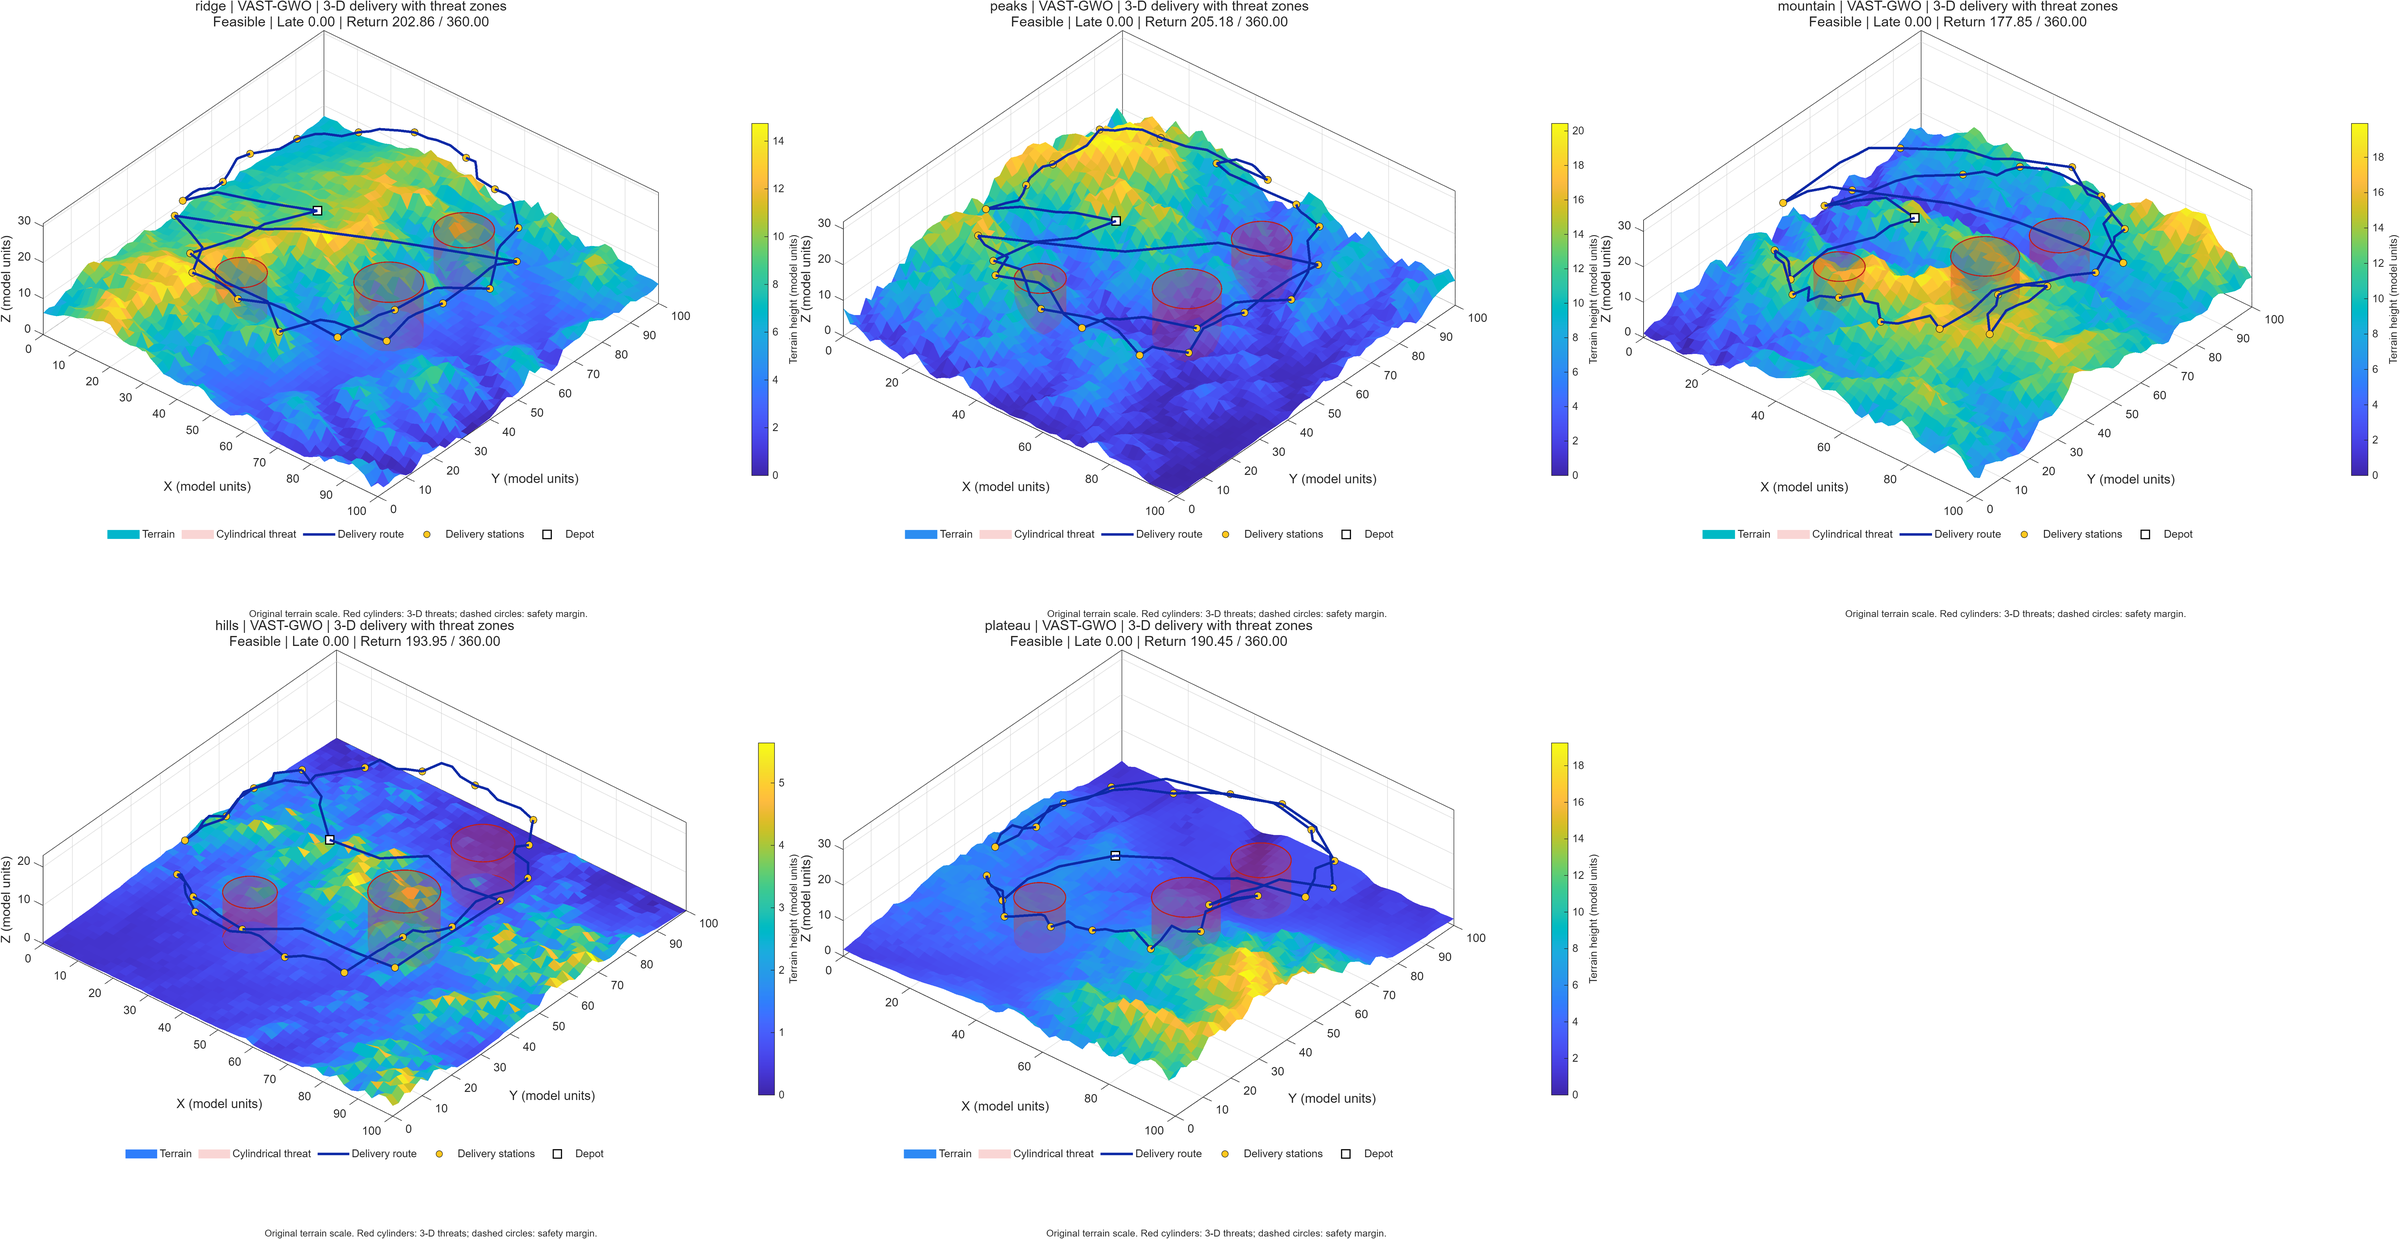
\includegraphics[width=\linewidth]{figures/uav_routes_montage.png}
\caption{Best feasible delivery routes found by \method{} on the five
DEM-based scenarios (costs 481.7--600.7). Terrain colour encodes elevation;
red cylinders are threat zones with safety margins; the blue polyline is the
route, dots are stations and the square is the depot.}
\label{fig:uavroutes}
\end{figure}

\subsection{Discussion of the application results}
The application reproduces the mechanism in a setting where the objective is
209-dimensional, the constraints are hard and the terrain is real: the method
that combines sparse evaluation with a verified multi-region archive is the
only one that is reliable on all five maps, it reaches feasibility faster than
every method except PSO---and that exception reverses by the end of the
budget---and it produces better final routes than all five baselines on the
paired runs where the comparison is meaningful. The trade-off that PSO
exhibits is instructive for practice: reaching any feasible route slightly
earlier is attractive in operations, but a method that then stalls at routes
19\% longer and misses 7 of 150 runs is a poor choice for a delivery plan. The
UAV results are therefore not an additional leaderboard but an independent
demonstration of the paper's central claim: with a scarce real-evaluation
budget, the composition of the candidate pool determines both whether feasible
solutions are found at all and how good they become.
\section{Discussion}
\label{sec:discussion}
\subsection{Candidate-source structure is a first-class design variable}
The experiments support a compact statement about optimizer design under
scarce real evaluations: \emph{the composition of the candidate pool is a
first-class design variable, and engineering it can outweigh engineering the
evaluation scheduler}. In \method{} that composition is a verified archive
spanning several regions of the search space. Because every archived centre is
backed by a billed evaluation, the archive can safely generate candidates far
from the current leaders without introducing unverified optimism; because it
spans multiple regions, it counteracts the leader-driven contraction that makes
GWO stagnate on multimodal landscapes; and because the allocation remains a
simple uniform draw, none of the gain depends on a fragile controller. The
boundary experiments make the contrast explicit: of the scheduling
mechanisms tested---directed screening, informed stratification, fixed quotas,
random quotas and three Q-learning policies---none improved on the uniform
draw, and the learned policies were never better than the best fixed policy.
This is a negative result that strengthens the paper's claim rather than
weakening it: it shows that the gain comes from the information the pool
contains, not from a particular way of spending the budget.

The behaviour metrics describe how the mechanism produces its effect.
\method{} recovers from stagnation windows more frequently than standard GWO
(0.823 against 0.757) and spends less of the budget inside long stagnation
(0.813 against 0.844). At the same time, its evaluations are individually more
valuable: the useful-novelty rate is almost twice that of standard GWO, and
the novelty rate in the final quarter remains high, which indicates that the
method continues to open new ground late in the run instead of refining a
single basin. These two observations correspond exactly to the dual objective
of the study---stagnation recovery and exploration efficiency under a fixed
true-evaluation budget---and both are measured from the same audit trail as
the final errors.

\subsection{Why the verified-state discipline matters}
Three of this paper's claims depend on the counting discipline rather than on
the algorithm alone. The comparison with strong baselines is meaningful only
if every method consumes exactly the same number of real evaluations, which is
why an independent probe audits every call. The ablation is meaningful only if
the evaluation budget, the pool size and the accepted-subset size are held
constant, which is why the disabled routes in the ablation are replaced by
standard candidates rather than removed. And the mechanism claim is meaningful
only if the archive contains measured information, which is why no unevaluated
candidate is allowed to influence leaders, archive or rankings. The same
discipline makes the method reproducible: the frozen configuration is
hash-identified, every configuration tested during development is retained
(including the ones that failed), and the formal batches are executed once
after freezing.

\subsection{Relation to the strong improved GWO}
The comparison with I-GWO deserves a precise reading. On the pooled statistic
the two methods are a tie, and the mean-rank advantage of \method{} is small
(2.24 against 2.28). The family decomposition shows why: \method{} leads on
unimodal, simple-multimodal and composition functions, while I-GWO retains an
advantage on hybrid functions. A defensible summary is therefore that the
method advances the state of the art in this comparison set---it is ranked
first among seven methods and is significantly better than five of
six---rather than that it dominates every competitor on every function. The
complementary structure also suggests a concrete direction for future work:
the hybrid functions, which combine subcomponents with different landscapes,
are exactly the case in which archive candidates could be complemented by a
stronger local search inside each subcomponent.

\subsection{Limitations and scope}
Four limitations bound the conclusions. First, the benchmark evidence covers
the CEC2017 suite at $D=50$ and $D=100$; whether the mechanism transfers to
thousands of dimensions or to constrained CEC suites remains open. Second, the
application evidence covers one family of terrain-constrained delivery
problems with hard time windows, simulated on five real terrain tiles; it is an
engineering-grade testbed, not a flight test. Third, the archive parameters
(capacity 24, separation threshold 2\% of the diagonal) were fixed from the
development phase and were not re-tuned per problem class; they behaved well
across the two dimensions and two budget levels tested here, but a broader
sensitivity study would be needed before deploying the method on problems with
very different geometry. Fourth, \method{} is the slowest method in wall-clock
time at equal budget ($1.6\times$ standard GWO), which is irrelevant when the
objective is expensive but should be weighed when it is not. None of these
limitations affects the paper's central claim, which concerns the composition
of the candidate pool rather than a claim of universal superiority.

\subsection{Future work}
Three directions follow directly from the results. First, the ablation
identifies a simpler configuration: because A2 is statistically
indistinguishable from the full method, a two-route variant that keeps only the
leader moves and the archive deserves a dedicated study, both for simplicity
and to test whether the archive alone can carry even more of the budget.
Second, the verified archive is a natural training set for a lightweight
surrogate, because every entry is a real measurement; coupling the two would
extend the method to objectives whose evaluations are expensive by orders of
magnitude. Third, the application evidence motivates delivery problems with
moving obstacles, stochastic time windows and multi-UAV fleets, where the
candidate pool would have to cover several vehicles simultaneously---a setting
in which the multi-region property of the archive should be even more valuable.

\section{Conclusion}
\label{sec:conclusion}
This paper introduced \method{}, a verified archive-guided sparse-evaluation
grey wolf optimizer for optimization under limited real-evaluation budgets.
The method separates cheap candidate generation---100 candidates from leader
moves, success-scale alpha shells and a verified multi-region elite
archive---from real evaluation, of which exactly ten uniformly drawn
candidates are paid for per generation, and admits only verified information
into the leaders, the archive and the rankings. On CEC2017 at $D=50$ with
100{,}000 probe-audited evaluations and 30 independent runs, \method{} attains
the best mean rank among seven methods, significantly outperforms five of the
six baselines---including a 2026 hierarchical GWO and a 2026 oppositional
GWO---and reaches statistical parity with the strongest classical improvement
while leading it on the rank summary. Controlled equal-slot ablations show
that the verified multi-region archive is the performance engine: a pool of
standard GWO moves alone loses 27 of the 29 functions to the full method, and
replacing the archive with a single-centre sampler with identical slots, scale
and acceptance rule collapses the method to 2 wins, whereas the alpha-shell
route becomes optional once the archive is present. The method holds its rank both at $D=100$ and with a budget five
times smaller, and every tested alternative scheduler---including three
Q-learning policies---failed to improve on the uniform draw. In a
209-dimensional DEM-based 3D UAV delivery application with hard time windows,
\method{} is the only method feasible in all 150 runs and achieves both the
best censored time to feasibility and the best paired final route quality
against every baseline.

The broader lesson is that when real evaluations are the scarce resource, the
structure of the candidate pool is a first-class design variable. Verifying
everything that enters memory, and generating candidates from several verified
regions, proved to be a more effective use of a fixed evaluation budget than
adding scheduling complexity. We hope this encourages future work to treat the
candidate pool, and the accounting of what enters the search state, as a
primary object of study in population-based optimization under expensive
evaluations.

\section*{Data and code availability}
All optimization and application experiments, including raw per-run records,
the experiment registry (every configuration and negative result), the
ablation implementation, the five UAV scenarios and the analysis scripts, are
available in the accompanying repository. The evaluation counts of all runs
are asserted by an independent probe, and the frozen method configuration is
bitwise audited against its archived implementation.

\bibliographystyle{unsrtnat}
\bibliography{references}

\end{document}
